\documentclass[11pt,letterpaper]{article}
\usepackage{fontspec}
\setmainfont{texgyrepagella}[Extension=.otf,UprightFont=*-regular,BoldFont=*-bold,ItalicFont=*-italic,BoldItalicFont=*-bolditalic]
\usepackage[bidi=default]{babel}
\babelprovide[import,main]{spanish}
\babelprovide[import]{hebrew}
\babelprovide[import]{ancientgreek}
\babelfont[hebrew]{rm}[Path=fonts/,BoldFont=NotoHebrewSerif-700.ttf,Scale=0.95]{NotoHebrewSerif-400.ttf}
\babelfont[ancientgreek]{rm}[Path=fonts/]{GFSPorson.otf}
\newcommand{\heb}[1]{\mbox{\foreignlanguage{hebrew}{#1}}}
\newcommand{\grc}[1]{\foreignlanguage{ancientgreek}{#1}}
\newcommand{\hebverso}[1]{\par\smallskip{\centering\begin{otherlanguage}{hebrew}\large #1\end{otherlanguage}\par}\smallskip}
\newcommand{\SENOR}{\textsc{Señor}}
\usepackage[margin=2.5cm,headheight=14pt]{geometry}
\usepackage{microtype,ragged2e,booktabs,graphicx,xcolor,csquotes,array}
\usepackage[hidelinks]{hyperref}\usepackage{xurl}\urlstyle{same}
\usepackage[most]{tcolorbox}
\usepackage{tikz}\usetikzlibrary{arrows.meta,positioning,calc,decorations.pathreplacing,shapes.geometric}
\usepackage{titlesec,fancyhdr}
\definecolor{tierraroja}{RGB}{122,40,18}\definecolor{caferojizo}{RGB}{58,18,8}
\definecolor{mostaza}{RGB}{214,160,58}\definecolor{papiro}{RGB}{243,228,192}\definecolor{sepia}{RGB}{98,66,44}
\definecolor{oliva}{RGB}{92,98,48}
\titleformat{\section}{\Large\bfseries\color{tierraroja}}{\thesection.}{0.6em}{}
\titleformat{\subsection}{\large\bfseries\color{caferojizo}}{\thesubsection}{0.6em}{}
\pagestyle{fancy}\fancyhf{}
\fancyhead[L]{\foreignlanguage{spanish}{\small\itshape\color{sepia}Yom Kipur}}\fancyhead[R]{\foreignlanguage{spanish}{\small\color{sepia}\thepage}}
\renewcommand{\headrulewidth}{0.4pt}
\setlength{\parindent}{1.27cm}\linespread{1.15}\setlength{\emergencystretch}{3em}
\newtcolorbox{cita}[1][]{enhanced,unbreakable,colback=tierraroja!5!white,colframe=tierraroja,boxrule=0pt,leftrule=2.5pt,arc=0pt,
  left=8pt,right=8pt,top=5pt,bottom=5pt,before skip=8pt,after skip=8pt,fontupper=\itshape,#1}
\newcommand{\fuente}[1]{\par\hfill{\upshape\bfseries\small\textcolor{tierraroja}{#1}}}
\newtcolorbox{nota}[1][]{enhanced,unbreakable,colback=mostaza!10,colframe=mostaza!85!tierraroja,boxrule=0.6pt,arc=2pt,
  fonttitle=\bfseries\small,coltitle=caferojizo,colbacktitle=mostaza!30,fontupper=\small,title={#1}}
\newtcolorbox{filologia}[1][]{enhanced,unbreakable,colback=white,colframe=tierraroja!45,boxrule=0.5pt,arc=2pt,
  fonttitle=\bfseries\small,coltitle=white,colbacktitle=tierraroja!80,fontupper=\small,title={Filología: #1}}
\newcommand{\refapa}[1]{\par{\RaggedRight\hangindent=1.27cm\hangafter=1\noindent #1\par}\vspace{4pt}}
\newcommand{\destacar}[1]{\textbf{\textcolor{tierraroja}{#1}}}
\newcolumntype{L}[1]{>{\RaggedRight\arraybackslash}p{#1}}

\title{\color{tierraroja}\bfseries Yom haKipurim: el día de las Expiaciones\\[4pt]\large\color{sepia}\mdseries ``En este día se hará expiación por vosotros\ldots{} y seréis limpios de todos vuestros pecados delante de \SENOR'' (Lv 16:30)}
\author{}\date{}
\begin{document}
\maketitle\thispagestyle{empty}

\begin{abstract}\noindent
El décimo día del mes séptimo es la única fecha del calendario de Levítico 23 en que el sumo sacerdote cruza el velo y la única convocación santa definida por el ayuno. Levítico 16 explica por qué: un Dios santo ha decidido que su tabernáculo resida ``entre ellos en medio de sus impurezas'' (Lv 16:16), y ese santuario contaminado necesita ser purgado una vez al año. El capítulo estudia el día con el método de la serie. La lectura histórica recorre el contexto de Nadab y Abiú, los ritos de eliminación del antiguo Cercano Oriente, el silencio de los libros históricos, el Segundo Templo (Ben Sira, Filón, Josefo, Qumrán, la Misná) y la destrucción del año 70. La filológica examina \emph{kipper}, \emph{kipurim}, \emph{kapóret}, \emph{jatat}, las tres palabras del pecado de Lv 16:21, \emph{nasá avón}, Azazel, \emph{inui néfesh} y \emph{shabat shabatón}, y su paso al griego (\emph{hilastērion}, \emph{hilasmós}). La textual compara el Texto Masorético con la Septuaginta, Qumrán y los Targumim; la literaria muestra el lugar central de Lv 16, el recorrido del sumo sacerdote de dentro hacia fuera y los dos machos cabríos como un solo acto. Se expone después la lectura de la serie: Cristo, Sumo Pontífice, concluye el juicio que comienza por la casa de Dios; su salida del santuario celestial coincide con la resurrección y la transformación, y el macho cabrío para Azazel figura a Satanás, el instigador, atado por mil años. La discusión presenta las demás lecturas con sus autores. La síntesis sostiene que Yom Kipur es el día en que Dios purifica su morada para seguir habitando con su pueblo.
\par\smallskip\noindent\textbf{Palabras clave:} Yom Kipur, Levítico 16, \emph{kipper}, \emph{kapóret}, Azazel, sumo sacerdote, Hebreos 9, 11QMelquisedec, Jubileo.\end{abstract}

\begin{nota}[Nota sobre el texto]
Las citas bíblicas en español son de la Reina-Valera 1960 (RVR1960), convención de esta serie; donde esa versión escribe ``Jehová'', aquí se escribe \SENOR, que traduce el tetragrama \heb{יהוה}. Cuando se ofrece una traducción literal del hebreo o del griego se indica ``(trad. propia)''. El hebreo sigue la \emph{Biblia Hebraica Stuttgartensia} (Códice de Leningrado); el griego, NA28 y la Septuaginta de Rahlfs-Hanhart. La Misná y el Talmud se citan por tratado y capítulo (Danby, 1933; Sefaria), y Qumrán según García Martínez (1992). Los conteos de palabras son propios: se hicieron por lema (número de Strong) sobre el Códice de Leningrado etiquetado morfológicamente y, para el griego, sobre el SBLGNT. Todo lo que es tradición rabínica, lectura tipológica, cálculo o hipótesis se marca como \emph{precisión}. Mis presentaciones anteriores sobre Yom Kipur se integran a lo largo del estudio.
\end{nota}

%===================================================================
\section{Introducción: un Dios santo en medio de un pueblo impuro}

El Levítico plantea una pregunta que el lector moderno rara vez se hace: ¿qué le ocurre a la casa de Dios cuando su pueblo peca? Según el libro, el pecado no queda encerrado en la conciencia del que lo comete; deja una marca en el lugar donde Dios habita. Por eso, después de describir los sacrificios (Lv 1--7), la consagración de los sacerdotes (Lv 8--10) y las impurezas de la vida corporal (Lv 11--15), dedica un capítulo entero a un rito que limpia el santuario mismo. La frase que lo explica está en Lv 16:16: el sumo sacerdote purificará ``el tabernáculo de reunión, el cual reside entre ellos en medio de sus impurezas''. Dios ha decidido quedarse en medio de un pueblo impuro, y para quedarse prescribe un día en que su morada sea limpiada.

Ese día es \heb{יוֹם הַכִּפֻּרִים} (\emph{Yom haKipurim}, Lv 23:27), ``el día de las expiaciones'', que la tradición abrevia \emph{Yom Kipur}. Es la sexta convocación del ciclo de Levítico 23 y la segunda del mes séptimo, entre el día del sonido de trompeta y la fiesta de las cabañas. A diferencia de las demás, se celebra con ayuno y no con banquete: ``afligiréis vuestras almas'' (Lv 16:29; 23:27). Es también la única fecha del año en que un ser humano entra detrás del velo, en el lugar santísimo, y pronuncia allí la confesión de todo Israel.

\begin{center}
\resizebox{\linewidth}{!}{%
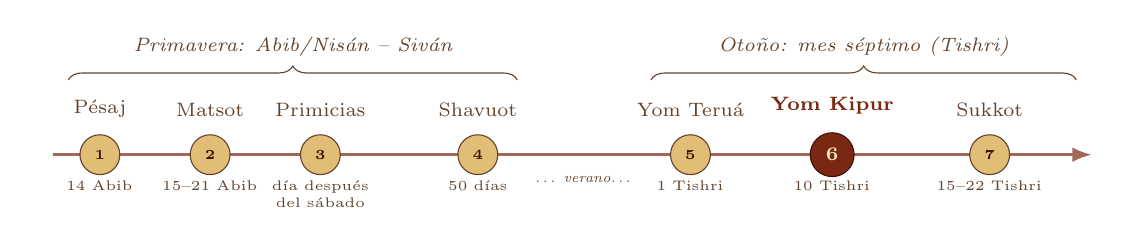
\begin{tikzpicture}[x=1cm,y=1cm,font=\scriptsize]
 \def\fiestaactual{6}
 \draw[line width=1.2pt,tierraroja!70,-{Latex[length=2.5mm]}] (0,0) -- (13.2,0);
 \draw[decorate,decoration={brace,amplitude=5pt},sepia] (0.2,0.95) -- (5.9,0.95) node[midway,above=5pt,font=\scriptsize\itshape]{Primavera: Abib/Nisán -- Siván};
 \draw[decorate,decoration={brace,amplitude=5pt},sepia] (7.6,0.95) -- (13.0,0.95) node[midway,above=5pt,font=\scriptsize\itshape]{Otoño: mes séptimo (Tishri)};
 \foreach \n/\x/\t/\d in {1/0.6/Pésaj/{14 Abib},2/2.0/Matsot/{15--21 Abib},3/3.4/Primicias/{día después del sábado},4/5.4/Shavuot/{50 días},5/8.1/Yom Teruá/{1 Tishri},6/9.9/Yom Kipur/{10 Tishri},7/11.9/Sukkot/{15--22 Tishri}}{
   \ifnum\n=\fiestaactual
     \node[circle,fill=tierraroja,draw=caferojizo,minimum size=5.5mm,text=papiro,font=\scriptsize\bfseries] at (\x,0) {\n};
     \node[above=3pt,font=\scriptsize\bfseries,text=tierraroja] at (\x,0.28) {\t};
   \else
     \node[circle,fill=mostaza!70,draw=sepia,minimum size=4.5mm,text=caferojizo,font=\tiny\bfseries] at (\x,0) {\n};
     \node[above=3pt,text=sepia] at (\x,0.25) {\t};
   \fi
   \node[below=6pt,text width=1.6cm,align=center,font=\tiny,text=sepia] at (\x,0) {\d};}
 \node[font=\tiny\itshape,text=sepia] at (6.75,-0.32) {\ldots\ verano\ldots};
\end{tikzpicture}}\par
{\footnotesize\color{sepia}\textit{Figura 1.} El ciclo de las convocaciones de Levítico 23: Yom Kipur, sexta convocación, el 10 del mes séptimo. \textit{Nota.} Elaboración propia.}
\end{center}

En mis presentaciones anteriores sobre la fiesta reuní los nombres con que el día ha sido llamado: el día de la expiación, el día ``cara a cara'', el Gran Día, el Ayuno, el día del gran shofar y el día del cierre de las puertas. Hace falta distinguir desde el comienzo cuáles nacen del texto bíblico y cuáles de la tradición posterior, porque esa distinción guiará todo el estudio.

\begin{center}\small\renewcommand{\arraystretch}{1.18}
\begin{tabular}{@{}L{3.3cm}L{6.4cm}L{5.0cm}@{}}
\toprule
\textbf{Nombre} & \textbf{Fundamento} & \textbf{Tipo de fuente} \\ \midrule
Día de las expiaciones & \heb{יוֹם הַכִּפֻּרִים}, Lv 23:27--28; 25:9 & bíblico \\
Sábado de reposo solemne & \heb{שַׁבַּת שַׁבָּתוֹן}, Lv 16:31; 23:32 & bíblico \\
El Ayuno & \grc{ἡ νηστεία}, Hch 27:9; Filón, \emph{Spec.} 2.193 & bíblico (NT) y judío helenista \\
El Día & \emph{Yomá}, ``el Día'' en arameo: nombre del tratado de la Misná & rabínico \\
Cara a cara & el sumo sacerdote ante la \emph{kapóret} (Lv 16:2); eco en 1~Co 13:12 & lectura devocional \\
El gran shofar & shofar del Jubileo en Yom Kipur (Lv 25:9); ``gran trompeta'' en Is 27:13 & bíblico (Lv 25:9); el vínculo con Is 27:13 es interpretativo \\
Cierre de las puertas & \emph{Neilá}, oración final; cf. Misná Taanit 4:1 & litúrgico posterior \\
\bottomrule
\end{tabular}\par
{\footnotesize\color{sepia}\textit{Tabla 1.} Los nombres del día. \textit{Nota.} Elaboración propia a partir de mis presentaciones anteriores.}
\end{center}

Sostengo en este estudio que \destacar{Yom Kipur es el día en que Dios purifica su morada para seguir habitando con su pueblo}, y que esa purificación tiene dos movimientos inseparables: la sangre que limpia el santuario de dentro hacia fuera y el macho cabrío vivo que se lleva las culpas lejos del campamento. El Nuevo Testamento lee ese día desde Cristo, el sumo sacerdote que entra ``una vez para siempre'' con su propia sangre y que ``aparecerá por segunda vez'' (He 9:12, 28). La serie da un paso más y ve en el día la conclusión del juicio que comienza por la casa de Dios, junto con la sentencia contra Satanás, el instigador del pecado.

El recorrido es el de toda la serie: primero el texto (Levítico 16 y los demás pasajes legales); luego las lecturas histórica, filológica, textual y literaria; después la lectura de la serie (memorial, figura y esperanza), la fiesta en Jesús y los apóstoles, la tradición judía y la discusión de interpretaciones, con especial atención a Azazel. Una síntesis y unas preguntas cierran el capítulo.

%===================================================================
\section{El texto}

\subsection{El contexto: la muerte de Nadab y Abiú}
Levítico 16 empieza con un funeral antes que con una fecha. ``Habló \SENOR{} a Moisés después de la muerte de los dos hijos de Aarón, cuando se acercaron delante de \SENOR, y murieron'' (Lv 16:1). El narrador remite al capítulo 10:

\begin{cita}Nadab y Abiú, hijos de Aarón, tomaron cada uno su incensario, y pusieron en ellos fuego, sobre el cual pusieron incienso, y ofrecieron delante de \SENOR{} fuego extraño, que él nunca les mandó. Y salió fuego de delante de \SENOR{} y los quemó, y murieron delante de \SENOR. Entonces dijo Moisés a Aarón: Esto es lo que habló \SENOR, diciendo: En los que a mí se acercan me santificaré, y en presencia de todo el pueblo seré glorificado. Y Aarón calló.\fuente{(Lv 10:1--3)}\end{cita}

Nadab y Abiú murieron por acercarse con incienso de un modo no prescrito; Lv 16 enseña a Aarón cómo acercarse con incienso de un modo prescrito, ``para que no muera'' (16:2, 13). El verbo \heb{קָרַב} (\emph{qarav}, ``acercarse'') une ambos textos: \heb{בְּקָרְבָתָם} (``cuando se acercaron'', 16:1) y \heb{בִּקְרֹבַי} (``en los que a mí se acercan'', 10:3). La pregunta del capítulo va más allá del perdón del pecado: cómo puede un hombre pecador entrar en la presencia de Dios y salir vivo.

\hebverso{וְאַל־יָבֹא בְכָל־עֵת אֶל־הַקֹּדֶשׁ מִבֵּית לַפָּרֹכֶת אֶל־פְּנֵי הַכַּפֹּרֶת אֲשֶׁר עַל־הָאָרֹן \\ וְלֹא יָמוּת כִּי בֶּעָנָן אֵרָאֶה עַל־הַכַּפֹּרֶת}
\begin{cita}Y \SENOR{} dijo a Moisés: Di a Aarón tu hermano, que no en todo tiempo entre en el santuario detrás del velo, delante del propiciatorio que está sobre el arca, para que no muera; porque yo apareceré en la nube sobre el propiciatorio.\fuente{(Lv 16:2)}\end{cita}

De esa restricción, ``no en todo tiempo'', nace el día. El acceso al lugar santísimo queda reducido a una fecha, una persona y un procedimiento, lo que Lv 16:34 resume en ``una vez al año''. Hebreos leerá ahí una lección del Espíritu Santo: mientras el primer tabernáculo estaba en pie, ``aún no se había manifestado el camino al Lugar Santísimo'' (He 9:8).

\subsection{Levítico 16: el rito paso a paso}
El capítulo puede leerse como un manual en ocho bloques.

\paragraph{1. Las vestiduras (v. 4).} Aarón deja las ``vestiduras sagradas\ldots{} para honra y hermosura'' de Éx 28:2 (efod, pectoral, manto con granadas, lámina de oro) y entra con cuatro piezas de lino blanco: ``Se vestirá la túnica santa de lino, y sobre su cuerpo tendrá calzoncillos de lino, y se ceñirá el cinto de lino, y con la mitra de lino se cubrirá. Son las santas vestiduras; con ellas se ha de vestir después de lavar su cuerpo con agua'' (Lv 16:4). El hebreo repite cuatro veces \heb{בַּד} (\emph{bad}, ``lino''). El lino sin adornos es la ropa de los ángeles en Ezequiel y Daniel (Ez 9:2; Dn 10:5); el sumo sacerdote se presenta vestido como un siervo y no como un príncipe.

\begin{nota}[Precisión sobre las vestiduras]
Algunas de mis láminas anteriores explican el día con las piezas de oro del sumo sacerdote (el efod con los nombres de las doce tribus, el pectoral, el Urim y el Tumim, la lámina ``Santidad a \SENOR''). Esa simbología es bíblica (Éx 28) y válida para el ministerio de Cristo, pero en Yom Kipur el rito interior se hacía con las vestiduras de lino; las de oro se vestían después, para los holocaustos (Lv 16:23--24). La Misná describe cinco inmersiones y diez lavados de manos y pies a lo largo del día (Misná Yomá 3:3), práctica del Segundo Templo y no del texto bíblico. La relación de las granadas del manto con los 613 mandamientos es una asociación popular; la cifra 613 procede del Talmud (b. Makot 23b).
\end{nota}

\paragraph{2. Los animales (vv. 3, 5--6).} Aarón aporta para sí ``un becerro para expiación, y un carnero para holocausto'' (v. 3); el pueblo aporta ``dos machos cabríos para expiación, y un carnero para holocausto'' (v. 5). Hay simetría: una \emph{jatat} y un holocausto por el sacerdote, una \emph{jatat} y un holocausto por el pueblo; y, dentro de esa simetría, los dos machos cabríos cuentan como una sola \emph{jatat}.

\paragraph{3. Las suertes (vv. 7--10).} Los dos machos se presentan ``delante de \SENOR{} a la puerta del tabernáculo de reunión'' y Aarón echa suertes sobre ellos:

\hebverso{וְנָתַן אַהֲרֹן עַל־שְׁנֵי הַשְּׂעִירִם גּוֹרָלוֹת גּוֹרָל אֶחָד לַיהוָה וְגוֹרָל אֶחָד לַעֲזָאזֵל}
\begin{cita}Y echará suertes Aarón sobre los dos machos cabríos; una suerte por \SENOR, y otra suerte por Azazel. Y hará traer Aarón el macho cabrío sobre el cual cayere la suerte por \SENOR, y lo ofrecerá en expiación. Mas el macho cabrío sobre el cual cayere la suerte por Azazel, lo presentará vivo delante de \SENOR{} para hacer la reconciliación sobre él, para enviarlo a Azazel al desierto.\fuente{(Lv 16:8--10)}\end{cita}

Las dos expresiones están construidas en paralelo: \heb{לַיהוָה} (\emph{laYHWH}, ``para \SENOR'') y \heb{לַעֲזָאזֵל} (\emph{laAzazel}, ``para Azazel''). La suerte, \heb{גּוֹרָל} (\emph{goral}), saca la elección de las manos humanas; es Dios quien decide cuál animal cumple cada función (cf. Pr 16:33).

\paragraph{4. El incienso (vv. 11--13).} Degollado el becerro, Aarón toma ``un incensario lleno de brasas de fuego del altar de delante de \SENOR, y sus puños llenos del perfume aromático molido, y lo llevará detrás del velo. Y pondrá el perfume sobre el fuego delante de \SENOR, y la nube del perfume cubrirá el propiciatorio que está sobre el testimonio, para que no muera'' (Lv 16:12--13). El incienso hace aquí lo que el fuego extraño de Nadab y Abiú no hizo: proteger al que entra, porque la nube de la \emph{ketóret} vela la nube de la gloria (16:2).

\paragraph{5. La sangre dentro del santuario (vv. 14--19).} Es el corazón del rito; la lectura literaria vuelve sobre él. Aarón rocía la sangre del becerro ``hacia el propiciatorio al lado oriental'' y ``siete veces'' delante de él (v. 14); hace lo mismo con la sangre del macho cabrío ``por el pecado del pueblo'' (v. 15); ``así purificará el santuario, a causa de las impurezas de los hijos de Israel, de sus rebeliones y de todos sus pecados; de la misma manera hará también al tabernáculo de reunión, el cual reside entre ellos en medio de sus impurezas'' (v. 16). Mientras tanto, ``ningún hombre estará en el tabernáculo de reunión'' (v. 17). Al salir, pone sangre en los cuernos del altar y lo rocía siete veces, ``y lo limpiará, y lo santificará de las inmundicias de los hijos de Israel'' (vv. 18--19).

\paragraph{6. El macho cabrío vivo (vv. 20--22).} Concluida la purificación del santuario, la tienda y el altar, empieza el segundo movimiento:

\hebverso{וְסָמַךְ אַהֲרֹן אֶת־שְׁתֵּי יָדָו עַל רֹאשׁ הַשָּׂעִיר הַחַי וְהִתְוַדָּה עָלָיו אֶת־כָּל־עֲוֺנֹת בְּנֵי יִשְׂרָאֵל \\ וְאֶת־כָּל־פִּשְׁעֵיהֶם לְכָל־חַטֹּאתָם וְנָתַן אֹתָם עַל־רֹאשׁ הַשָּׂעִיר וְשִׁלַּח בְּיַד־אִישׁ עִתִּי הַמִּדְבָּרָה}
\begin{cita}Cuando hubiere acabado de expiar el santuario y el tabernáculo de reunión y el altar, hará traer el macho cabrío vivo; y pondrá Aarón sus dos manos sobre la cabeza del macho cabrío vivo, y confesará sobre él todas las iniquidades de los hijos de Israel, todas sus rebeliones y todos sus pecados, poniéndolos así sobre la cabeza del macho cabrío, y lo enviará al desierto por mano de un hombre destinado para esto.\fuente{(Lv 16:20--21)}\end{cita}

\begin{cita}Y aquel macho cabrío llevará sobre sí todas las iniquidades de ellos a tierra inhabitada; y dejará ir el macho cabrío por el desierto.\fuente{(Lv 16:22)}\end{cita}

Es el único rito del Pentateuco en que se imponen las dos manos sobre un animal y se confiesa sobre él. Al animal no se lo sacrifica; se lo ``envía'' (\heb{שִׁלַּח}, \emph{shilaj}, tres veces en vv. 10, 21, 22). El que lo conduce es un \heb{אִישׁ עִתִּי} (\emph{ish ití}), literalmente ``un hombre del momento'', preparado o designado para la ocasión; la RVR1960 traduce ``destinado para esto'' y el documento de referencia cita ``un hombre preparado para esto''.

\paragraph{7. El cierre (vv. 23--28).} Aarón entra en la tienda, se quita las vestiduras de lino ``y las pondrá allí'', se lava ``en el lugar del santuario'', se viste sus ropas y ofrece los dos holocaustos (vv. 23--25). Siguen dos instrucciones de pureza que pesarán en la discusión sobre Azazel:

\begin{cita}El que hubiere llevado el macho cabrío a Azazel, lavará sus vestidos, lavará también con agua su cuerpo, y después entrará en el campamento. Y sacarán fuera del campamento el becerro y el macho cabrío inmolados por el pecado, cuya sangre fue llevada al santuario para hacer la expiación; y quemarán en el fuego su piel, su carne y su estiércol. El que los quemare lavará sus vestidos, lavará también su cuerpo con agua, y después podrá entrar en el campamento.\fuente{(Lv 16:26--28)}\end{cita}

\paragraph{8. El estatuto (vv. 29--34).} Solo al final aparece la fecha, y con ella el rito sacerdotal se convierte en día del pueblo:

\hebverso{כִּי־בַיּוֹם הַזֶּה יְכַפֵּר עֲלֵיכֶם לְטַהֵר אֶתְכֶם מִכֹּל חַטֹּאתֵיכֶם לִפְנֵי יְהוָה תִּטְהָרוּ}
\begin{cita}Y esto tendréis por estatuto perpetuo: En el mes séptimo, a los diez días del mes, afligiréis vuestras almas, y ninguna obra haréis, ni el natural ni el extranjero que mora entre vosotros. Porque en este día se hará expiación por vosotros, y seréis limpios de todos vuestros pecados delante de \SENOR. Día de reposo es para vosotros, y afligiréis vuestras almas; es estatuto perpetuo.\fuente{(Lv 16:29--31)}\end{cita}

El versículo 30 termina con un verbo, \heb{תִּטְהָרוּ} (\emph{titharu}, ``seréis puros''), y en él desemboca todo el aparato de sangre, incienso y suertes: la pureza del pueblo ``delante de \SENOR''. Los versículos 32--34 aseguran la continuidad; lo hará ``el sacerdote que fuere ungido'' en lugar de Aarón, ``una vez al año''.

\begin{center}
\resizebox{\linewidth}{!}{%
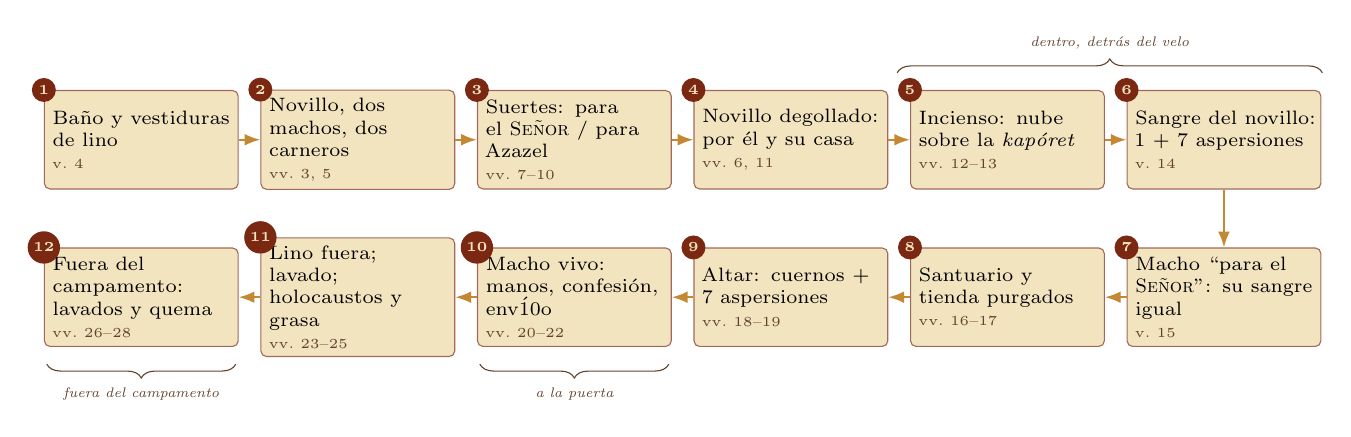
\begin{tikzpicture}[font=\scriptsize,
  paso/.style={draw=tierraroja!70,fill=papiro,rounded corners=2pt,text width=2.25cm,minimum height=1.25cm,align=left,inner sep=3pt},
  num/.style={circle,fill=tierraroja,text=papiro,font=\tiny\bfseries,inner sep=1.3pt},
  fl/.style={-{Latex[length=2mm]},mostaza!80!tierraroja,line width=0.8pt}]
 \foreach \i/\x/\y/\t/\r in {
  1/0/0/{Baño y vestiduras de lino}/{v.~4},
  2/2.75/0/{Novillo, dos machos, dos carneros}/{vv.~3, 5},
  3/5.5/0/{Suertes: para el \SENOR{} / para Azazel}/{vv.~7--10},
  4/8.25/0/{Novillo degollado: por él y su casa}/{vv.~6, 11},
  5/11.0/0/{Incienso: nube sobre la \emph{kapóret}}/{vv.~12--13},
  6/13.75/0/{Sangre del novillo: 1 + 7 aspersiones}/{v.~14},
  7/13.75/-2.0/{Macho ``para el \SENOR'': su sangre igual}/{v.~15},
  8/11.0/-2.0/{Santuario y tienda purgados}/{vv.~16--17},
  9/8.25/-2.0/{Altar: cuernos + 7 aspersiones}/{vv.~18--19},
  10/5.5/-2.0/{Macho vivo: manos, confesión, envío}/{vv.~20--22},
  11/2.75/-2.0/{Lino fuera; lavado; holocaustos y grasa}/{vv.~23--25},
  12/0/-2.0/{Fuera del campamento: lavados y quema}/{vv.~26--28}}{
  \node[paso] (p\i) at (\x,\y) {\RaggedRight \t\par{\tiny\color{sepia}\r}};
  \node[num] at (p\i.north west) {\i};}
 \foreach \a/\b in {1/2,2/3,3/4,4/5,5/6,7/8,8/9,9/10,10/11,11/12} \draw[fl] (p\a) -- (p\b);
 \draw[fl] (p6) -- (p7);
 \draw[decorate,decoration={brace,amplitude=5pt},sepia] (9.6,0.85) -- (15.0,0.85) node[midway,above=5pt,font=\tiny\itshape]{dentro, detrás del velo};
 \draw[decorate,decoration={brace,amplitude=5pt,mirror},sepia] (4.3,-2.85) -- (6.7,-2.85) node[midway,below=5pt,font=\tiny\itshape]{a la puerta};
 \draw[decorate,decoration={brace,amplitude=5pt,mirror},sepia] (-1.2,-2.85) -- (1.2,-2.85) node[midway,below=5pt,font=\tiny\itshape]{fuera del campamento};
\end{tikzpicture}}\par
{\footnotesize\color{sepia}\textit{Figura 2.} La secuencia ritual de Levítico 16 en doce pasos. \textit{Nota.} Elaboración propia sobre el texto de Lv 16 (RVR1960).}
\end{center}

\subsection{Levítico 23:26--32: el día del pueblo}
Lv 16 mira el día desde el santuario; Lv 23 lo mira desde el pueblo, en el calendario de las ``fiestas solemnes de \SENOR, las cuales proclamaréis como santas convocaciones'' (23:2):

\hebverso{אַךְ בֶּעָשׂוֹר לַחֹדֶשׁ הַשְּׁבִיעִי הַזֶּה יוֹם הַכִּפֻּרִים הוּא מִקְרָא־קֹדֶשׁ יִהְיֶה לָכֶם \\ וְעִנִּיתֶם אֶת־נַפְשֹׁתֵיכֶם וְהִקְרַבְתֶּם אִשֶּׁה לַיהוָה}
\begin{cita}A los diez días de este mes séptimo será el día de expiación; tendréis santa convocación, y afligiréis vuestras almas, y ofreceréis ofrenda encendida a \SENOR. Ningún trabajo haréis en este día; porque es día de expiación, para reconciliaros delante de \SENOR{} vuestro Dios. Porque toda persona que no se afligiere en este mismo día, será cortada de su pueblo.\fuente{(Lv 23:27--29)}\end{cita}

\begin{cita}Y cualquiera persona que hiciere trabajo alguno en este día, yo destruiré a la tal persona de entre su pueblo. Ningún trabajo haréis; estatuto perpetuo es por vuestras generaciones en dondequiera que habitéis. Día de reposo será a vosotros, y afligiréis vuestras almas, comenzando a los nueve días del mes en la tarde; de tarde a tarde guardaréis vuestro reposo.\fuente{(Lv 23:30--32)}\end{cita}

Tres rasgos distinguen este pasaje de los demás del capítulo. Es el único que amenaza con el \emph{karet}, ``será cortada de su pueblo'' (v. 29), y con la destrucción directa por Dios (``yo destruiré'', v. 30). Es el único que repite tres veces \heb{בְּעֶצֶם הַיּוֹם הַזֶּה} (``en este mismo día'', vv. 28, 29, 30), como para impedir que el día se traslade. Y es el único que fija el comienzo y el final: \heb{בְּתִשְׁעָה לַחֹדֶשׁ בָּעֶרֶב מֵעֶרֶב עַד־עֶרֶב} (``a los nueve días del mes en la tarde; de tarde a tarde'', v. 32). La partícula inicial \heb{אַךְ} (\emph{aj}, ``pero'', ``solamente'', v. 27) marca el contraste con la fiesta alegre que lo precede. En cuanto al \emph{karet}, no se trata de una pena ejecutada por el tribunal sino de una sanción que Dios se reserva, la extinción del linaje o la exclusión del pueblo (Milgrom, 2001).

\subsection{Los demás textos legales}
Números 29:7--11 fija las ofrendas del día: un becerro, un carnero y siete corderos en holocausto, ``un macho cabrío por expiación; además de la ofrenda de las expiaciones por el pecado, y del holocausto continuo'' (v. 11). Esa última frase distingue la \emph{jatat} ordinaria del día de la \heb{חַטַּאת הַכִּפֻּרִים} (\emph{jatat hakipurim}) de Lv 16. Éxodo 30:10 anticipa el rito al describir el altar del incienso: ``sobre sus cuernos hará Aarón expiación una vez en el año con la sangre del sacrificio por el pecado para expiación''. Y Levítico 25:9 hace del día el punto de partida del Jubileo: ``Entonces harás tocar fuertemente la trompeta en el mes séptimo a los diez días del mes; el día de la expiación haréis tocar la trompeta por toda vuestra tierra'' (cf. el estudio 09, \emph{El Jubileo}).

\begin{center}\small\renewcommand{\arraystretch}{1.2}
\begin{tabular}{@{}L{2.2cm}L{4.4cm}L{8.2cm}@{}}
\toprule
\textbf{Texto} & \textbf{Perspectiva} & \textbf{Qué añade} \\ \midrule
Éx 30:10 & el altar del incienso & expiación anual sobre sus cuernos con ``la sangre del sacrificio por el pecado para expiación'' (\emph{jatat hakipurim}) \\
Lv 16:1--28 & el santuario y el sumo sacerdote & la entrada tras el velo, las vestiduras de lino, las suertes, la sangre sobre la \emph{kapóret}, el macho vivo, los lavados \\
Lv 16:29--34 & el calendario & 10 del mes séptimo; afligir el alma; ninguna obra; \emph{shabat shabatón}; natural y extranjero; ``estatuto perpetuo''; ``una vez al año'' \\
Lv 23:26--32 & el pueblo convocado & \emph{mikrá kódesh}; \emph{karet} y destrucción; ``en este mismo día'' (3 veces); ``de tarde a tarde'' \\
Lv 25:8--10 & el ciclo de años & el shofar del año 50 suena en Yom Kipur; ``pregonaréis libertad'' (\emph{derór}) \\
Nm 29:7--11 & las ofrendas públicas & holocausto (1 becerro, 1 carnero, 7 corderos), \emph{jatat} adicional, holocausto continuo \\
\bottomrule
\end{tabular}\par
{\footnotesize\color{sepia}\textit{Tabla 2.} Tabla sinóptica de los textos legales sobre Yom Kipur. \textit{Nota.} Elaboración propia; Deuteronomio 16, que enumera las fiestas de peregrinación, no menciona el día.}
\end{center}

El silencio de Deuteronomio tiene explicación. Dt 16 legisla las tres fiestas de peregrinación (Pésaj, Shavuot, Sukkot), en las que el pueblo ``se presenta'' en el lugar escogido; Yom Kipur no pertenece a ese grupo, porque el pueblo ayuna ``en dondequiera que habitéis'' (Lv 23:31) mientras el sumo sacerdote actúa en su nombre. Hebreos construirá sobre esa distribución de papeles.

%===================================================================
\section{Lectura histórica}

\subsection{El mes séptimo en el año agrícola}
El décimo día del mes séptimo cae entre fines de septiembre y comienzos de octubre, un tiempo de bisagra en el año de Israel: las cosechas de grano están guardadas, la vendimia y la recolección de frutos están por terminar, y la tierra espera las primeras lluvias (la \emph{yoré}, Dt 11:14; Jl 2:23) que ablandarán el suelo para la nueva siembra. El documento de referencia lo describe bien: ``al llegar al séptimo mes, entonces, la cosecha final del año ya está guardada en el alfolí'', y los veintidós días que van de Trompetas al último gran día de Cabañas son ``un tiempo de consagración a Dios''. Yom Kipur ocupa el centro de ese período; el pueblo se detiene, ayuna y queda limpio antes de la alegría de la fiesta de la cosecha (Lv 23:39--40).

El calendario marítimo del Mediterráneo confirma la fecha desde otro ángulo. Lucas anota que, en el viaje de Pablo a Roma, ``siendo ya peligrosa la navegación, por haber pasado ya el ayuno'' (Hch 27:9). Para los navegantes antiguos la temporada segura terminaba a mediados de septiembre y el mar se cerraba hacia noviembre, de modo que ``el ayuno'' sirve a Lucas como marca de calendario conocida por sus lectores.

\begin{nota}[Precisión cronológica]
La fecha exacta del ayuno de Hch 27:9 depende del año del viaje, que suele situarse hacia el 59 o 60 e.\,c. Algunos comentaristas calculan que en el 59 el 10 de Tishri cayó a comienzos de octubre; es un cálculo con márgenes, porque el inicio del mes dependía de la observación de la luna nueva y de la eventual intercalación de un mes.
\end{nota}

\subsection{Ritos de eliminación en el antiguo Cercano Oriente}
Israel no fue el único pueblo que purificaba templos y expulsaba males. Los textos hititas describen ritos en que un animal (un carnero, una cabra, a veces adornada) se envía al territorio enemigo cargado con la peste o el mal que afecta al ejército; en Babilonia, durante las ceremonias de año nuevo (\emph{akītu}) del mes de Nisán, un sacerdote purificaba el santuario de Nabû frotándolo con el cadáver de un carnero (\emph{kuppuru}, verbo emparentado con el hebreo \emph{kipper}) que luego se arrojaba al río, y los oficiantes debían salir al campo y quedarse allí hasta el fin de la fiesta (Wright, 1987; Milgrom, 1991).

Los paralelos iluminan la forma del rito y, al mismo tiempo, hacen visibles sus diferencias. En Lv 16 no hay conjuro ni divinidad que aplacar con el animal enviado; el macho cabrío no se ofrece a Azazel, y el texto insiste en que ambos animales se presentan ``delante de \SENOR'' (vv. 7, 10). Lo que se elimina tampoco es una peste ni un demonio, sino ``las iniquidades\ldots{} rebeliones y\ldots{} pecados'' confesados por el pueblo (v. 21). Milgrom resume la diferencia diciendo que el Levítico conserva una forma antigua pero la vacía de magia y la llena de moral (Milgrom, 1991). Para el método de la serie la lección es sobria: el contexto ayuda a ver lo que el texto comparte con su mundo y, sobre todo, lo que se niega a compartir.

\subsection{La fiesta en la historia narrada de Israel}
Ningún libro histórico del Antiguo Testamento narra una celebración de Yom Kipur, lo que sorprende en una fiesta de este peso. Hay indicios cercanos:
\begin{itemize}\setlength{\itemsep}{1pt}
\item Salomón dedica el templo ``en el mes de Etanim, que es el mes séptimo'' y celebra catorce días de fiesta (1~R 8:2, 65--66; 2~Cr 7:8--10). La tradición rabínica se preguntó si ese año se ayunó en Yom Kipur y concluyó que no (b. Moed Katán 9a): es una inferencia talmúdica, no un dato del texto.
\item Al volver del exilio, el altar se reconstruye ``llegado el mes séptimo'' y se ofrecen holocaustos ``desde el primer día del mes séptimo'' (Esd 3:1--6), pero no se menciona el día décimo.
\item En Nehemías 8 se lee la Ley el primer día del mes séptimo y se celebra Sukkot; el ayuno colectivo de Neh 9:1 ocurre el día 24, no el 10.
\end{itemize}
El silencio no prueba que el día no se guardara; muestra que los narradores no lo usaron como escenario. La serie, en cambio, propone leer en la historia de Israel el ``hito'' que el día conmemora: el fin del juicio en el desierto antes de entrar en la tierra (véase §\ref{sec:serie}).

\subsection{El Segundo Templo}
A partir del siglo~\textsc{ii} a.\,e.\,c. las fuentes se multiplican y el día pasa a ocupar el centro de la piedad judía.

\paragraph{Ben Sira 50.} El elogio del sumo sacerdote Simón, hijo de Onías (ca. 200 a.\,e.\,c.), describe su salida del santuario: ``¡Qué glorioso era\ldots{} cuando salía de la casa del velo!'' (Si 50:5, trad. propia; \grc{ἐν ἐξόδῳ οἴκου καταπετάσματος}). Las comparaciones con la estrella de la mañana, el sol y el arco iris (50:6--7) dicen el alivio y la alegría del pueblo al ver salir vivo al sacerdote.

\begin{nota}[Precisión]
Muchos intérpretes leen Si 50:5--21 como una escena de Yom Kipur, porque solo ese día el sumo sacerdote salía de ``la casa del velo''. Otros sostienen que describe el sacrificio diario (\emph{tamid}), con el que coinciden varios detalles del final (las libaciones, las trompetas, la bendición; Hayward, 1996). El pasaje sirve aquí como testimonio de la emoción ligada a la \emph{salida} del sumo sacerdote, sin decidir el debate.
\end{nota}

\paragraph{Jubileos.} El libro de los Jubileos (s.~\textsc{ii} a.\,e.\,c.) da al día un origen histórico: los hijos de Jacob degollaron un cabrito, mancharon con su sangre la túnica de José y engañaron a su padre el día 10 del mes séptimo; por eso Israel debe afligirse ese día y expiar sus pecados ``con un cabrito'' (Jub 34:12--19). Es una lectura memorial antigua, distinta de la de la serie pero del mismo tipo, pues busca en la historia un hecho que el día recuerde.

\paragraph{Qumrán.} El \emph{Pésher de Habacuc} conserva un dato valioso: el Sacerdote Impío persiguió al Maestro de Justicia ``a su lugar de destierro'' y ``en el tiempo de la fiesta del reposo del Día de las Expiaciones'' se presentó ante ellos para devorarlos y hacerlos tropezar ``en el día de ayuno, sábado de su reposo'' (1QpHab XI 4--8; trad. según García Martínez, 1992). La expresión hebrea \heb{מועד מנוחת יום הכפורים} (``la fiesta del reposo del Día de las Expiaciones'') muestra que el día seguía siendo, a la vez, ayuno y sábado. El \emph{Rollo del Templo} reelabora el rito de Lv 16 (11Q19 XXV 10 -- XXVII 10), y el texto llamado 11QMelquisedec lo proyecta al fin de los tiempos (véase §\ref{sec:mesias}).

\begin{nota}[Precisión: el calendario de Qumrán]
Que el Sacerdote Impío pudiera atacar al Maestro en su Yom Kipur, día en que un sumo sacerdote de Jerusalén estaría oficiando en el templo, sugiere que ambos grupos guardaban el día en fechas distintas. Es la hipótesis habitual: la comunidad seguía un calendario solar de 364 días, distinto del lunisolar del templo (VanderKam, 1998).
\end{nota}

\paragraph{Filón y Josefo.} Filón de Alejandría (ca. 20 a.\,e.\,c. -- 50 e.\,c.) llama al día simplemente ``el Ayuno'' (\grc{νηστεία}) y lo cuenta entre las fiestas: una fiesta sin comida ni bebida, en que el alma se nutre de oración y de dominio propio, guardada incluso por quienes descuidan las demás prácticas (\emph{De specialibus legibus} 1.186--188; 2.193--203). Josefo describe el rito con el macho enviado ``a un lugar desierto, más allá de las fronteras'' como expiación por el pueblo (\emph{Antigüedades} 3.240--243) y cuenta que Pompeyo tomó el templo en el 63 a.\,e.\,c. ``en el día del ayuno'' (\emph{Antigüedades} 14.66).

\begin{nota}[Precisión]
En \emph{Ant.} 14.66 algunos entienden ``el día del ayuno'' como Yom Kipur y otros como un sábado (los autores grecorromanos creían que los judíos ayunaban en sábado). El dato es útil para mostrar que ``el Ayuno'' era nombre corriente del día, no para fechar con certeza la conquista.
\end{nota}

\paragraph{La Misná.} El tratado \emph{Yomá} (``el Día''), compilado hacia el 200 e.\,c., describe con minucia el servicio del Segundo Templo: la separación del sumo sacerdote siete días antes, las tres confesiones, la caja de las suertes, la cinta escarlata y la lectura de la Torá. Es fuente posterior a la destrucción del templo y mezcla memoria histórica con normativa rabínica; se estudia en §\ref{sec:tradicion}.

\paragraph{La destrucción del año 70.} Con el templo desaparecieron el sumo sacerdote, la \emph{kapóret} (ya ausente desde la destrucción del primer templo) y el macho para Azazel; el día sobrevivió como ayuno, oración y confesión. Una tradición talmúdica afirma que ``durante los cuarenta años anteriores a la destrucción del templo'' la suerte ``para el \SENOR'' no salió en la mano derecha y la cinta escarlata no se volvió blanca (b. Yomá 39b). En mis láminas destaqué ese dato, porque esos cuarenta años coinciden aproximadamente con el tiempo transcurrido desde la crucifixión. Hay que decir, sin embargo, que es una tradición rabínica tardía, transmitida como \emph{baraita}, y que la conexión con Jesús es lectura cristiana posterior; vale como dato de memoria judía y no como prueba.

\begin{center}
\resizebox{\linewidth}{!}{%
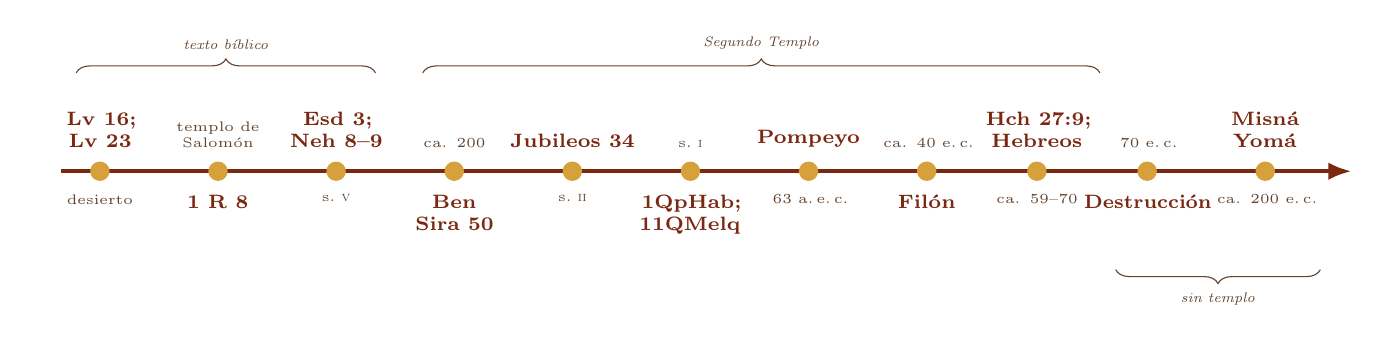
\begin{tikzpicture}[font=\scriptsize]
 \draw[line width=1.6pt,tierraroja,-{Latex[length=3mm]}] (0,0) -- (16.4,0);
 \foreach \x/\a/\b/\s in {
   0.5/{Lv 16; Lv 23}/{desierto}/1,
   2.0/{1 R 8}/{templo de Salomón}/-1,
   3.5/{Esd 3; Neh 8--9}/{s.~\textsc{v}}/1,
   5.0/{Ben Sira 50}/{ca. 200}/-1,
   6.5/{Jubileos 34}/{s.~\textsc{ii}}/1,
   8.0/{1QpHab; 11QMelq}/{s.~\textsc{i}}/-1,
   9.5/{Pompeyo}/{63 a.\,e.\,c.}/1,
   11.0/{Filón}/{ca. 40 e.\,c.}/-1,
   12.4/{Hch 27:9; Hebreos}/{ca. 59--70}/1,
   13.8/{Destrucción}/{70 e.\,c.}/-1,
   15.3/{Misná Yomá}/{ca. 200 e.\,c.}/1}{
   \fill[mostaza] (\x,0) circle (3.5pt);
   \ifnum\s=1
     \node[above=5pt,font=\scriptsize\bfseries,text=tierraroja,text width=1.6cm,align=center] at (\x,0) {\a};
     \node[below=5pt,text width=1.6cm,align=center,font=\tiny,text=sepia] at (\x,0) {\b};
   \else
     \node[below=5pt,font=\scriptsize\bfseries,text=tierraroja,text width=1.6cm,align=center] at (\x,0) {\a};
     \node[above=5pt,text width=1.6cm,align=center,font=\tiny,text=sepia] at (\x,0) {\b};
   \fi}
 \draw[decorate,decoration={brace,amplitude=5pt},sepia] (0.2,1.25) -- (4.0,1.25) node[midway,above=5pt,font=\tiny\itshape]{texto bíblico};
 \draw[decorate,decoration={brace,amplitude=5pt},sepia] (4.6,1.25) -- (13.2,1.25) node[midway,above=5pt,font=\tiny\itshape]{Segundo Templo};
 \draw[decorate,decoration={brace,amplitude=5pt,mirror},sepia] (13.4,-1.25) -- (16.0,-1.25) node[midway,below=5pt,font=\tiny\itshape]{sin templo};
\end{tikzpicture}}\par
{\footnotesize\color{sepia}\textit{Figura 3.} Yom Kipur en las fuentes: del texto bíblico a la Misná. \textit{Nota.} Elaboración propia; fechas aproximadas.}
\end{center}

%===================================================================
\section{Lectura filológica}

El vocabulario de Lv 16 es denso y técnico. Varias de sus palabras son raras (\emph{Azazel}, \emph{ish ití} y \emph{érets guezerá} aparecen solo aquí) y otras, muy frecuentes, alcanzan en este capítulo su sentido más pleno. Los recuadros que siguen estudian las principales en su raíz, sus usos concretos, su paso a la Septuaginta y su eco en el Nuevo Testamento (Brown, Driver y Briggs, 1906; Koehler y Baumgartner, 2001; Bauer et al., 2000).

\begin{filologia}[\heb{כִּפֶּר} \emph{kipper}]
La raíz \heb{כ־פ־ר} aparece 102 veces en forma verbal (conteo propio por lema sobre el Códice de Leningrado: 49 en Levítico y 16 en Lv 16). El único uso en la forma simple (\emph{qal}) es concreto: Noé ``la calafatearás con brea por dentro y por fuera'' (\heb{וְכָפַרְתָּ אֹתָהּ \foreignlanguage{spanish}{[\ldots]} בַּכֹּפֶר}, Gn 6:14). La forma intensiva \emph{kipper} es el verbo de la expiación. Los estudiosos discuten su sentido básico:
\begin{itemize}\setlength{\itemsep}{0pt}
\item \textbf{Cubrir}: por Gn 6:14 y el árabe \emph{kafara}. Es la explicación tradicional (``cubrir el pecado''), hoy menos aceptada para los textos rituales.
\item \textbf{Rescatar}: por el sustantivo \heb{כֹּפֶר} (\emph{kófer}), ``rescate'', el precio que sustituye una vida (Éx 21:30; 30:12; Nm 35:31; Sal 49:7 [49:8]). Éx 30:16 llama a la ofrenda del censo \heb{כֶּסֶף הַכִּפֻּרִים} (``el dinero de las expiaciones''), ``para hacer expiación por vuestras personas''.
\item \textbf{Purgar, limpiar}: por el acadio \emph{kuppuru}, ``frotar, limpiar ritualmente''. Milgrom (1991) sostiene que en los textos de la \emph{jatat} \emph{kipper} significa ``purgar'' y que su objeto propio es el santuario, no el pecador; Levine (1989) prefiere ``limpiar, borrar'' (\emph{to wipe off}).
\end{itemize}
La sintaxis de Lv 16 apoya que el verbo tenga varias caras: con complemento directo, se purgan cosas (\heb{כִּפֶּר אֶת־הַקֹּדֶשׁ}, ``expiar el santuario'', vv. 20, 33); con \heb{בְּעַד} (\emph{be'ad}, ``a favor de''), se expía por personas (vv. 6, 11, 17, 24); con \heb{עַל} (\emph{al}), ``sobre'' o ``por'' (vv. 10, 16, 18, 30, 34). La Septuaginta traduce casi siempre \grc{ἐξιλάσκομαι}.
\end{filologia}

\begin{nota}[Precisión: el debate sobre la purgación]
Milgrom (1991) propuso que cada pecado e impureza del año contamina el santuario a distancia, como un miasma, y que el sacrificio por el pecado (\emph{jatat}) limpia el santuario y no al pecador; Yom Kipur limpiaría la contaminación acumulada en las zonas interiores, adonde las ofrendas ordinarias no llegan. Gane (2005) discute ese esquema: durante el año la \emph{jatat} purifica al oferente, y la culpa ya perdonada queda en el santuario, que Dios ``carga''; en Yom Kipur Dios purga su propia morada de esas faltas ya perdonadas, en un segundo tiempo de la expiación. Ambos coinciden en que el día limpia el santuario y en que la limpieza tiene consecuencias para el pueblo (Lv 16:30).
\end{nota}

\begin{filologia}[\heb{יוֹם הַכִּפֻּרִים} \emph{yom hakipurim}]
\emph{Kipurim} es un sustantivo plural derivado de \emph{kipper}. Aparece ocho veces, siempre en plural (Éx 29:36; 30:10, 16; Lv 23:27, 28; 25:9; Nm 5:8; 29:11; conteo propio). El plural no indica varios actos, sino una noción abstracta e intensiva, como en \emph{miluím} (``consagración'', Éx 29:22) o \emph{bikurim} (``primicias''): ``la expiación'' en sentido pleno. La RVR1960 alterna ``día de expiación'' (Lv 23:27) y ``día de la expiación'' (Lv 25:9); el documento de referencia lo llama ``día de las expiaciones'', más cerca del plural hebreo. La Septuaginta dice \grc{ἡμέρα ἐξιλασμοῦ} (Lv 23:27). El nombre moderno \emph{Yom Kipur} es la forma abreviada, en singular, de la tradición judía.
\end{filologia}

\begin{filologia}[\heb{כַּפֹּרֶת} \emph{kapóret}]
La tapa de oro puro que cubría el arca, con los dos querubines ``de una pieza'' con ella (Éx 25:17--22). Aparece 27 veces, siete de ellas en Lv 16 (vv. 2 [dos veces], 13, 14 [dos], 15 [dos]; conteo propio). El nombre viene de la misma raíz que \emph{kipper}: no es una simple tapa (para eso existía \heb{מִכְסֶה}), sino el lugar de la expiación. Es también el lugar del encuentro: ``Y de allí me declararé a ti, y hablaré contigo de sobre el propiciatorio'' (Éx 25:22; cf. Nm 7:89). La Septuaginta la llama \grc{ἱλαστήριον ἐπίθεμα} (``cubierta propiciatoria'', Éx 25:17) y luego simplemente \grc{τὸ ἱλαστήριον}; la Vulgata, \emph{propitiatorium}; de ahí el español ``propiciatorio''. En el Nuevo Testamento, \grc{ἱλαστήριον} designa la \emph{kapóret} en He 9:5 y se aplica a Cristo en Ro 3:25. Primera de Crónicas 28:11 llama al lugar santísimo \heb{בֵּית הַכַּפֹּרֶת}, ``la casa del propiciatorio''.
\end{filologia}

\begin{filologia}[\heb{חַטָּאת} \emph{jatat} y \heb{עֹלָה} \emph{olá}]
\heb{חַטָּאת} significa a la vez ``pecado'' y el sacrificio que lo trata (14 apariciones en Lv 16, con ambos sentidos; conteo propio). La RVR1960 traduce ``expiación'' o ``sacrificio por el pecado''. Milgrom (1991) propone ``ofrenda de purificación'', porque la exige también una impureza sin culpa moral: la mujer que da a luz (Lv 12:6--8), el leproso sanado (14:19), el nazareo que tocó un muerto (Nm 6:11). La forma verbal \emph{jitté} significa ``des-pecar'', es decir, purificar: ``Purifícame con hisopo, y seré limpio'' (\heb{תְּחַטְּאֵנִי}, Sal 51:7 [51:9]). \heb{עֹלָה} (\emph{olá}), de \heb{עָלָה} (``subir''), es el holocausto, la ofrenda que ``sube'' entera en humo; en Lv 16 cierra el día (v. 24).
\end{filologia}

\subsection{Las tres palabras del pecado}
La confesión sobre el macho vivo usa los tres términos principales del pecado en el Antiguo Testamento, cada uno con su imagen concreta:

\begin{filologia}[\heb{עָוֺן} \emph{avón}, \heb{פֶּשַׁע} \emph{pésha}, \heb{חַטָּאת} \emph{jatat}]
\textbf{\emph{Avón}} viene de una raíz que significa ``torcer, doblar''; designa la iniquidad, la culpa que queda y también su castigo: ``Grande es mi castigo (\heb{עֲוֺנִי}) para ser soportado'', dice Caín (Gn 4:13). \textbf{\emph{Pésha}} es la rebelión, la ruptura de una relación de lealtad: el verbo se usa para Israel que ``se apartó'' de la casa de David (1~R 12:19) y para Edom que ``se rebeló'' contra Judá (2~R 8:20). En todo el Levítico \emph{pésha} solo aparece en Lv 16:16, 21 (conteo propio). \textbf{\emph{Jatá}} (con su sustantivo \emph{jatat}) es ``errar el blanco'': los honderos de Benjamín ``tiraban una piedra con la honda a un cabello, y no erraban'' (\heb{וְלֹא יַחֲטִא}, Jue 20:16). Juntas, las tres palabras abarcan toda falta: la torcida, la rebelde y la fallida. La misma tríada aparece en la revelación del Nombre: Dios ``perdona la iniquidad, la rebelión y el pecado'' (\heb{נֹשֵׂא עָוֺן וָפֶשַׁע וְחַטָּאָה}, Éx 34:7).
\end{filologia}

\begin{center}
\begin{tikzpicture}[font=\small,
  pal/.style={draw=tierraroja!70,fill=papiro,rounded corners=3pt,text width=3.4cm,align=center,inner sep=4pt},
  fl/.style={-{Latex[length=2mm]},mostaza!80!tierraroja,line width=0.9pt}]
 \node[pal] (a) at (0,2.3) {\heb{עֲוֺנֹת} \emph{avonot}\\ \footnotesize ``iniquidades''\\ \scriptsize\color{sepia} torcer: culpa que pesa};
 \node[pal] (p) at (4.8,2.3) {\heb{פְּשָׁעִים} \emph{peshaím}\\ \footnotesize ``rebeliones''\\ \scriptsize\color{sepia} romper la lealtad};
 \node[pal] (j) at (9.6,2.3) {\heb{חַטֹּאת} \emph{jatot}\\ \footnotesize ``pecados''\\ \scriptsize\color{sepia} errar el blanco};
 \node[draw=tierraroja,line width=0.9pt,fill=tierraroja!8,rounded corners=3pt,text width=7.4cm,align=center,inner sep=5pt] (c) at (4.8,0.0)
   {\heb{וְהִתְוַדָּה עָלָיו}\\ ``confesará sobre él''\\[2pt] \heb{וְנָתַן אֹתָם עַל־רֹאשׁ הַשָּׂעִיר}\\ ``poniéndolos así sobre la cabeza''\\ \scriptsize\color{sepia}(Lv 16:21)};
 \node[pal,text width=7.4cm] (d) at (4.8,-2.75) {\heb{וְנָשָׂא הַשָּׂעִיר עָלָיו} \ \ \heb{אֶל־אֶרֶץ גְּזֵרָה}\\ ``llevará sobre sí'' \ldots{} ``a tierra inhabitada''\\ \scriptsize\color{sepia}(Lv 16:22)};
 \draw[fl] (a) -- (c); \draw[fl] (p) -- (c); \draw[fl] (j) -- (c); \draw[fl] (c) -- (d);
 \node[font=\scriptsize\itshape,text=sepia,text width=13cm,align=center] at (4.8,-3.95) {La misma tríada: Éx 34:7 (Dios ``perdona'', \emph{nosé}); Sal 32:1--2; Dn 9:24.};
\end{tikzpicture}\par
{\footnotesize\color{sepia}\textit{Figura 4.} Las tres palabras del pecado en Lv 16:21--22 y su destino. \textit{Nota.} Elaboración propia; hebreo según la BHS.}
\end{center}

\begin{filologia}[\heb{נָשָׂא עָוֺן} \emph{nasá avón}]
``Llevar la iniquidad'' tiene dos sentidos en la Biblia hebrea. Puede significar \emph{cargar con la culpa propia} y su castigo: el que oye un juramento y no denuncia ``llevará su pecado'' (Lv 5:1), y la generación que rechazó la tierra oye: ``llevaréis vuestras iniquidades cuarenta años'' (\heb{תִּשְׂאוּ אֶת־עֲוֺנֹתֵיכֶם}, Nm 14:34). Puede significar también \emph{quitar la culpa de otro}, es decir, perdonar: Dios es \heb{נֹשֵׂא עָוֺן} (Éx 34:7; Nm 14:18; Mi 7:18). Los sacerdotes comen la \emph{jatat} ``para llevar la iniquidad de la congregación'' (Lv 10:17). En Lv 16:22 el sujeto es el macho cabrío: \heb{וְנָשָׂא הַשָּׂעִיר עָלָיו אֶת־כָּל־עֲוֺנֹתָם}. El Siervo de Isaías hace lo mismo: ``llevará las iniquidades de ellos'' (53:11) y ``habiendo él llevado (\heb{נָשָׂא}) el pecado de muchos'' (53:12). La Septuaginta de Is 53:12 traduce \grc{ἀνήνεγκεν}, el verbo que Hebreos usa para Cristo, ``ofrecido una sola vez para llevar (\grc{ἀνενεγκεῖν}) los pecados de muchos'' (He 9:28; cf. 1~P 2:24).
\end{filologia}

\begin{filologia}[\heb{עֲזָאזֵל} \emph{Azazel}]
El nombre aparece solo cuatro veces, todas en Lv 16 (vv. 8, 10 [dos veces], 26; conteo propio). Su sentido es uno de los problemas clásicos del Pentateuco. Hay cuatro grandes hipótesis:
\begin{enumerate}\setlength{\itemsep}{0pt}
\item \textbf{``El macho que se va''}: se lee \heb{עֵז אֹזֵל} (\emph{ez ozel}, ``cabra que se va''). Es la interpretación de la Septuaginta (\grc{ἀποπομπαῖος}, ``el que es enviado lejos''), de Símaco y de la Vulgata (\emph{caper emissarius}); de ella vienen el inglés \emph{scapegoat} (Tyndale, 1530) y el español ``chivo expiatorio''.
\item \textbf{Un lugar escarpado}: el Sifra, el Talmud (b. Yomá 67b, ``el más duro de los montes'') y el Targum Pseudo-Jonatán entienden un lugar áspero del desierto; la Misná describe el despeñadero al que se llevaba el animal (Misná Yomá 6:6--8). G.~R. Driver (1956) apoyó la idea con el árabe \emph{azāz}, ``terreno áspero''.
\item \textbf{Un ser demoníaco del desierto}: lo sugiere el paralelo \heb{לַיהוָה} / \heb{לַעֲזָאזֵל}, que pide dos personas. En 1~Enoc, Azazel (o Asael) es el jefe de los vigilantes caídos que enseñó a los hombres las armas y los adornos, y Dios ordena atarlo y arrojarlo a las tinieblas en el desierto (1~En 8:1; 10:4--8); en el \emph{Apocalipsis de Abraham} (caps. 13--14) es una figura satánica. Defienden esta lectura Milgrom (1991), Levine (1989) y Hartley (1992), con matices.
\item \textbf{Un nombre abstracto}: ``remoción total'', de una raíz \emph{azal} ``quitar'' (Brown, Driver y Briggs, 1906).
\end{enumerate}
Un dato literario acompaña la tercera lectura: los machos cabríos son \heb{שְׂעִירִם} (\emph{se'irim}, Lv 16:5), y el capítulo siguiente prohíbe ofrecer sacrificios ``a los demonios'', también \heb{שְּׂעִירִם} (Lv 17:7; cf. Is 13:21; 34:14). La discusión completa, con la lectura de la serie, está en §\ref{sec:azazel}.
\end{filologia}

\begin{filologia}[\heb{עִנָּה נֶפֶשׁ} \emph{inui néfesh}]
``Afligiréis vuestras almas'' (\heb{וְעִנִּיתֶם אֶת־נַפְשֹׁתֵיכֶם}, Lv 16:29, 31; 23:27, 32; Nm 29:7). El verbo \emph{inná} es ``humillar, doblegar''; \heb{נֶפֶשׁ} (\emph{néfesh}) designa en su sentido concreto la garganta y el apetito: ``el alma hambrienta'' (Sal 107:9), el Seol que, como una garganta, ``ensanchó su \emph{néfesh}'' (Is 5:14, trad. propia; RVR1960: ``su interior''). Afligir la \emph{néfesh} es, ante todo, negarle el alimento. Los textos paralelos lo confirman: ``afligí con ayuno mi alma'' (\heb{עִנֵּיתִי בַצּוֹם נַפְשִׁי}, Sal 35:13); ``¿Por qué, dicen, ayunamos, y no hiciste caso; humillamos nuestras almas, y no te diste por entendido?'' (Is 58:3); Esdras proclama ayuno ``para afligirnos delante de nuestro Dios'' (Esd 8:21). El documento de referencia y el folleto de la Iglesia de Dios Unida lo entienden así, con Sal 35:13 y 69:10 [69:11]. La Septuaginta traduce \grc{ταπεινώσετε τὰς ψυχὰς ὑμῶν}. La Misná precisa cinco abstenciones: comer y beber, lavarse, ungirse, calzar sandalias y las relaciones conyugales (Misná Yomá 8:1), precisión rabínica.
\end{filologia}

\begin{filologia}[\heb{שַׁבַּת שַׁבָּתוֹן} \emph{shabat shabatón}]
La construcción repite el sustantivo para formar un superlativo, como ``lugar santísimo'' (\emph{kódesh kodashim}) o ``cantar de los cantares'': ``reposo de reposo absoluto''. La expresión se aplica solo al sábado semanal (Éx 31:15; 35:2; Lv 23:3), a Yom Kipur (Lv 16:31; 23:32) y al año sabático (Lv 25:4). Las demás convocaciones son \emph{shabatón} (Lv 23:24, 39) y prohíben ``obra de siervos'' (\heb{מְלֶאכֶת עֲבֹדָה}, 23:7, 8, 21, 25, 35, 36); Yom Kipur, como el sábado, prohíbe ``todo trabajo'' (\heb{כָּל־מְלָאכָה}, 23:28, 30, 31). La Septuaginta dice \grc{σάββατα σαββάτων}. De ahí que el documento de referencia lo llame ``un sábado santo establecido como mandato por Dios''.
\end{filologia}

\begin{filologia}[\heb{קְטֹרֶת} \emph{ketóret}]
El incienso, de una raíz que significa ``hacer humo''. Su fórmula era exclusiva del santuario (Éx 30:34--38); en Lv 16:12 se pide \heb{קְטֹרֶת סַמִּים דַּקָּה}, ``perfume aromático molido''. Su nube cubre la \emph{kapóret} ``para que no muera'' (16:13). La Escritura asocia el incienso con la oración: ``Suba mi oración delante de ti como el incienso'' (Sal 141:2); la multitud oraba fuera ``a la hora del incienso'' (Lc 1:10), y en el Apocalipsis el incienso sube con ``las oraciones de todos los santos'' (Ap 8:3--4; cf. 5:8). Mis láminas anteriores destacan esta línea, que es bíblica.
\end{filologia}

\begin{filologia}[\heb{אִישׁ עִתִּי} \emph{ish ití} y \heb{אֶרֶץ גְּזֵרָה} \emph{érets guezerá}]
Ambas expresiones son únicas en la Biblia hebrea. \emph{Ití} viene de \heb{עֵת} (``tiempo''): ``un hombre del momento'', preparado para la ocasión; la Septuaginta traduce \grc{ἀνθρώπου ἑτοίμου} (``un hombre preparado''), de donde la versión que cita el documento de referencia. \emph{Guezerá} viene de \heb{גָּזַר}, ``cortar'': Salomón ordena ``partid'' al niño (1~R 3:25), Dios ``dividió el mar Rojo en partes'' (Sal 136:13). La ``tierra cortada'' es tierra separada, sin retorno; la RVR1960 traduce ``tierra inhabitada'' y la Septuaginta \grc{εἰς γῆν ἄβατον} (``tierra intransitable''). El mismo verbo describe al Siervo: ``fue cortado (\heb{נִגְזַר}) de la tierra de los vivientes'' (Is 53:8).
\end{filologia}

\subsection{Del hebreo al griego del Nuevo Testamento}
La Septuaginta tradujo la familia de \emph{kipper} con la familia griega de \grc{ἱλάσκομαι}, y esa elección pasó al Nuevo Testamento:

\begin{filologia}[Vocabulario griego]
\begin{tabular}{@{}L{3.4cm}L{11.2cm}@{}}
\grc{ἀποπομπαῖος} & ``el que es enviado lejos'': la Septuaginta de Lv 16:8, 10 traduce así \emph{laAzazel}; en 16:10 dice además \grc{εἰς τὴν ἀποπομπήν} (``para el envío'') y en 16:26 \grc{εἰς ἄφεσιν} (``para la liberación''). \\[2pt]
\grc{ἐξιλάσκομαι}, \grc{ἐξιλασμός} & ``expiar'', ``expiación'': traducen \emph{kipper} y \emph{kipurim} (Lv 16:30; 23:27). \\[2pt]
\grc{ἱλάσκομαι} & ``hacer propicio, expiar'': Cristo, ``misericordioso y fiel sumo sacerdote\ldots{} para expiar (\grc{εἰς τὸ ἱλάσκεσθαι}) los pecados del pueblo'' (He 2:17); el publicano: ``Dios, sé propicio a mí, pecador'' (\grc{ἱλάσθητί μοι}, Lc 18:13). \\[2pt]
\grc{ἱλαστήριον} & la \emph{kapóret} (He 9:5) y Cristo, ``a quien Dios puso como propiciación'' (Ro 3:25). \\[2pt]
\grc{ἱλασμός} & ``propiciación'': ``él es la propiciación por nuestros pecados'' (1~Jn 2:2); Dios ``envió a su Hijo en propiciación'' (1~Jn 4:10). \\[2pt]
\grc{ἀρχιερεύς} & ``sumo sacerdote'': 17 veces en Hebreos (conteo propio), donde la RV1909 decía ``pontífice'', término que conserva el documento de referencia. \\[2pt]
\grc{ἡ νηστεία} & ``el ayuno'': nombre del día en Hch 27:9, Filón y Josefo. \\
\end{tabular}
\end{filologia}

\begin{center}
\begin{tikzpicture}[font=\small,
  cad/.style={draw=tierraroja!70,fill=papiro,rounded corners=3pt,text width=3.2cm,align=center,inner sep=5pt,minimum height=2.3cm},
  fl/.style={-{Latex[length=2.2mm]},mostaza!80!tierraroja,line width=1pt}]
 \node[cad] (h) at (0,0) {\textbf{Hebreo}\\[2pt] \heb{כִּפֶּר} \emph{kipper}\\ \heb{כִּפֻּרִים} \emph{kipurim}\\ \heb{כַּפֹּרֶת} \emph{kapóret}};
 \node[cad] (s) at (4.1,0) {\textbf{Septuaginta}\\[2pt] \grc{ἐξιλάσκομαι}\\ \grc{ἐξιλασμός}\\ \grc{ἱλαστήριον}};
 \node[cad] (n) at (8.2,0) {\textbf{Nuevo Testamento}\\[2pt] \grc{ἱλάσκεσθαι} (He 2:17)\\ \grc{ἱλασμός} (1~Jn 2:2)\\ \grc{ἱλαστήριον} (Ro 3:25; He 9:5)};
 \node[cad] (e) at (12.3,0) {\textbf{Español}\\[2pt] expiar\\ propiciación\\ propiciatorio};
 \draw[fl] (h) -- (s); \draw[fl] (s) -- (n); \draw[fl] (n) -- (e);
 \node[font=\scriptsize\itshape,text=sepia,text width=15cm,align=center] at (6.15,-1.75) {La tapa del arca y la persona de Cristo comparten un nombre: el lugar donde Dios trata el pecado para seguir habitando con su pueblo.};
\end{tikzpicture}\par
{\footnotesize\color{sepia}\textit{Figura 5.} De \emph{kipper} a \emph{hilastérion}. \textit{Nota.} Elaboración propia.}
\end{center}

%===================================================================
\section{Lectura textual}

\subsection{Levítico 16 en el Texto Masorético y la Septuaginta}
El texto hebreo de Lv 16 es estable; los manuscritos de Qumrán que conservan Levítico y el Pentateuco Samaritano no presentan variantes que alteren el rito. Las diferencias importantes están en la traducción, sobre todo donde las versiones antiguas tuvieron que decidir qué era Azazel.

\begin{center}\small\renewcommand{\arraystretch}{1.2}
\begin{tabular}{@{}L{1.4cm}L{4.2cm}L{4.6cm}L{4.4cm}@{}}
\toprule
\textbf{Verso} & \textbf{TM (BHS)} & \textbf{Septuaginta} & \textbf{Lectura implicada} \\ \midrule
16:8 & \heb{גּוֹרָל אֶחָד לַעֲזָאזֵל} & \grc{κλῆρον ἕνα τῷ ἀποπομπαίῳ} & ``una suerte para el enviado lejos'': Azazel = el macho mismo \\
16:10a & \heb{הַגּוֹרָל לַעֲזָאזֵל} & \grc{ὁ κλῆρος τοῦ ἀποπομπαίου} & ídem \\
16:10b & \heb{לְשַׁלַּח אֹתוֹ לַעֲזָאזֵל הַמִּדְבָּרָה} & \grc{ἀποστεῖλαι αὐτὸν εἰς τὴν ἀποπομπήν} & ``para el envío'': Azazel = la acción de alejar \\
16:21 & \heb{בְּיַד־אִישׁ עִתִּי} & \grc{ἐν χειρὶ ἀνθρώπου ἑτοίμου} & ``un hombre preparado'' \\
16:22 & \heb{אֶל־אֶרֶץ גְּזֵרָה} & \grc{εἰς γῆν ἄβατον} & ``tierra intransitable'' \\
16:26 & \heb{אֶת־הַשָּׂעִיר לַעֲזָאזֵל} & \grc{τὸν χίμαρον τὸν διεσταλμένον εἰς ἄφεσιν} & ``el designado para la liberación'' \\
\bottomrule
\end{tabular}\par
{\footnotesize\color{sepia}\textit{Tabla 3.} Azazel en el Texto Masorético y en la Septuaginta. \textit{Nota.} Elaboración propia; Septuaginta según Rahlfs-Hanhart.}
\end{center}

La Septuaginta no transcribe el nombre; lo interpreta, y de tres modos distintos en el mismo capítulo. Ninguno supone un demonio, porque el traductor alejandrino vio en Azazel el \emph{alejamiento} mismo. Su elección en 16:26 tiene consecuencias teológicas, ya que \grc{ἄφεσις} es la palabra con que la misma versión traduce el Jubileo (Lv 25:10--13) y la que el Nuevo Testamento usa para el perdón (``remisión de pecados'', Mt 26:28; Ef 1:7) y para la libertad anunciada por Jesús en Nazaret (Lc 4:18). El Targum de Onquelos conserva ``para Azazel''; el Targum Pseudo-Jonatán lo explica como un lugar ``duro y áspero'' del desierto (Lv 16:10). Ya en la Antigüedad, por tanto, conviven las tres lecturas principales: un nombre propio, una acción y un lugar.

\begin{nota}[Precisión textual]
\textbf{Lv 16:21}. El texto consonántico dice \heb{ידו}, que por sí solo podría leerse ``su mano''; los masoretas indican leer \heb{יָדָיו} (``sus manos''), como exige el numeral \heb{שְׁתֵּי} (``dos''). La RVR1960 sigue la lectura masorética: ``sus dos manos''. Es el único rito en que se imponen las \emph{dos} manos, gesto que la Misná entiende como transferencia y confesión (Misná Yomá 6:2).\par\smallskip
\textbf{Lv 16:10}. La frase \heb{לְכַפֵּר עָלָיו} puede entenderse ``para hacer expiación \emph{sobre} él'' (RVR1960: ``para hacer la reconciliación sobre él'') o ``por medio de él''. La Septuaginta dice \grc{ἐξιλάσασθαι ἐπ᾿ αὐτοῦ}. El texto no explica cómo un animal no sacrificado participa en la expiación; los comentarios proponen que el macho vivo queda incluido en el acto expiatorio del día por haber sido presentado ``delante de \SENOR'' (Hartley, 1992; Milgrom, 1991).\par\smallskip
\textbf{Lv 16:18}. ``El altar que está delante de \SENOR'' es para la mayoría de los comentaristas modernos el altar exterior de los holocaustos (Milgrom, 1991); la Misná lo identificó con el altar de oro del incienso (Misná Yomá 5:5), lectura que recogí en mis láminas y que encuentra apoyo en Éx 30:10.
\end{nota}

\subsection{Daniel 9:24: \emph{lekaper avón}}
La profecía de las setenta semanas reúne el vocabulario de Yom Kipur:

\hebverso{שָׁבֻעִים שִׁבְעִים נֶחְתַּךְ עַל־עַמְּךָ וְעַל־עִיר קָדְשֶׁךָ לְכַלֵּא הַפֶּשַׁע וּלְהָתֵם חַטָּאת וּלְכַפֵּר עָוֺן \\ וּלְהָבִיא צֶדֶק עֹלָמִים וְלַחְתֹּם חָזוֹן וְנָבִיא וְלִמְשֹׁחַ קֹדֶשׁ קָדָשִׁים}
\begin{cita}Setenta semanas están determinadas sobre tu pueblo y sobre tu santa ciudad, para terminar la prevaricación, y poner fin al pecado, y expiar la iniquidad, para traer la justicia perdurable, y sellar la visión y la profecía, y ungir al Santo de los santos.\fuente{(Dn 9:24)}\end{cita}

Vuelven las tres palabras de Lv 16:21 (\emph{pésha}, \emph{jatat}, \emph{avón}) con el verbo \heb{לְכַפֵּר} (``expiar''), y la frase final, ``ungir al Santo de los santos'', remite al santuario. El documento de referencia cita este texto para decir que el Mesías se sacrifica ``para expiar la iniquidad de la humanidad, como le fuera revelado al profeta Daniel''.

\begin{nota}[Precisión textual y cronológica]
En Dn 9:24 el texto consonántico dice \heb{ולחתם חטאות} (``y para sellar los pecados''), y los masoretas indican leer \heb{וּלְהָתֵם חַטָּאת} (``y para poner fin al pecado''); la RVR1960 sigue la segunda lectura. En cuanto al cálculo, las ``setenta semanas'' (490 años) se han contado desde distintos decretos persas (Ciro, 538; Artajerjes, 458/457 o 445/444 a.\,e.\,c.) para llegar al ministerio o la muerte de Jesús, mientras que la mayoría de los estudios críticos las refiere a la crisis de Antíoco IV (167--164 a.\,e.\,c.). Ninguno de esos cómputos está explícito en el texto; son lecturas.
\end{nota}

\subsection{Romanos 3:25: ¿propiciatorio o propiciación?}
\begin{cita}\ldots{}a quien Dios puso como propiciación por medio de la fe en su sangre, para manifestar su justicia, a causa de haber pasado por alto, en su paciencia, los pecados pasados.\fuente{(Ro 3:25)}\end{cita}

El griego dice \grc{ὃν προέθετο ὁ θεὸς ἱλαστήριον διὰ [τῆς] πίστεως ἐν τῷ αὐτοῦ αἵματι}. El debate tiene dos niveles. El primero es el referente de \grc{ἱλαστήριον}: si Pablo alude a la \emph{kapóret} de Yom Kipur (``propiciatorio''), como en He 9:5 y en la mayoría de sus usos en el Pentateuco griego, o usa la palabra en sentido general (``medio de propiciación''), como en 4~Macabeos 17:22, donde la muerte de los mártires es \grc{ἱλαστήριον} por Israel. Dunn (1998) ve en el versículo el lenguaje del sacrificio por el pecado y del día de la expiación; Moo (1996) considera probable la alusión a la \emph{kapóret}, aunque advierte que el lector de Roma podía entender el término sin conocer la liturgia del templo. Si la alusión es correcta, Cristo queda presentado como el lugar del encuentro y de la expiación que en Lv 16 estaba oculto tras el velo, ahora ``puesto'' a la vista (\grc{προέθετο}).

El segundo nivel es el sentido de la raíz, ``expiación'' (quitar el pecado) o ``propiciación'' (aplacar la ira). Dodd (1935) sostuvo que en la Septuaginta la familia de \grc{ἱλάσκομαι} perdió el sentido de aplacar y significa ``expiar''; Morris (1955) respondió que el contexto de ira divina (Ro 1:18; 2:5) conserva el sentido de propiciación. La RVR1960, con ``propiciación'', sigue la segunda tradición. Muchos intérpretes actuales sostienen que en el texto bíblico ambos sentidos se implican, porque el pecado expiado es el pecado que provocaba la ira.

\subsection{Hebreos 9:4 y el altar de oro}
Hebreos sitúa en el lugar santísimo un \grc{χρυσοῦν θυμιατήριον} (He 9:4). La RVR1960 traduce ``un incensario de oro''; otros entienden ``el altar de oro del incienso'', que según Éx 30:6 estaba \emph{delante} del velo. Dos datos aclaran la aparente contradicción: el incensario de Lv 16:12 entraba precisamente ese día detrás del velo, y 1~R 6:22 llama al altar del incienso \heb{הַמִּזְבֵּחַ אֲשֶׁר־לַדְּבִיר}, ``el altar que pertenecía al santuario interior'' (trad. propia). El autor de Hebreos describe el tabernáculo desde Yom Kipur, y desde ese día el altar del incienso pertenece funcionalmente al lugar santísimo, porque su humo es el que entra (Attridge, 1989; Lane, 1991).

\subsection{``Pecados de ignorancia'': Hebreos 9:7}
``Pero en la segunda parte, sólo el sumo sacerdote una vez al año, no sin sangre, la cual ofrece por sí mismo y por los pecados de ignorancia del pueblo'' (He 9:7). La palabra \grc{ἀγνοήματα} reduce el alcance del día a las faltas no deliberadas, en línea con Lv 4--5 y Nm 15:22--31, donde el pecado ``con soberbia'' (literalmente ``con mano alzada'') no tiene sacrificio. Lv 16, sin embargo, incluye también las ``rebeliones'' (\emph{peshaím}, vv. 16, 21). El documento de referencia sigue a Hebreos cuando dice que el Sumo Pontífice intercede ``por los pecados involuntarios y de ignorancia de su pueblo''; la Misná sigue a Levítico cuando afirma que Yom Kipur expía también faltas graves, a condición del arrepentimiento (Misná Yomá 8:8).

\subsection{``De tarde a tarde'': el cómputo del día}
Lv 23:32 es el texto de la Torá que con mayor claridad fija el comienzo de un día sagrado al atardecer: el día 10 se guarda ``comenzando a los nueve días del mes en la tarde; de tarde a tarde''. Lo destaqué en mis láminas, y la serie lo aplica al sábado y a todas las convocaciones. La tradición judía hizo de esta frase la base para comenzar el ayuno antes de la puesta del sol (b. Yomá 81b). Cuándo cae el día en el calendario civil depende del cómputo del mes; el calendario rabínico fijo (codificado hacia el siglo~\textsc{iv} e.\,c.) impide que Yom Kipur caiga en viernes o domingo, para no unir dos días de reposo absoluto, regla posterior y no bíblica.

%===================================================================
\section{Lectura literaria}

\subsection{Levítico 16 en el centro del Levítico}
Varios autores han propuesto que el Levítico tiene una estructura concéntrica y que Lv 16 ocupa su centro (Douglas, 1999; Warning, 1999). La propuesta varía en los detalles (otros sitúan el centro en el capítulo 19, con ``amarás a tu prójimo como a ti mismo''), pero ayuda a ver la función del capítulo, que une la primera mitad del libro, centrada en el santuario y los sacerdotes, con la segunda, centrada en la santidad del pueblo, del tiempo y de la tierra.

\begin{center}
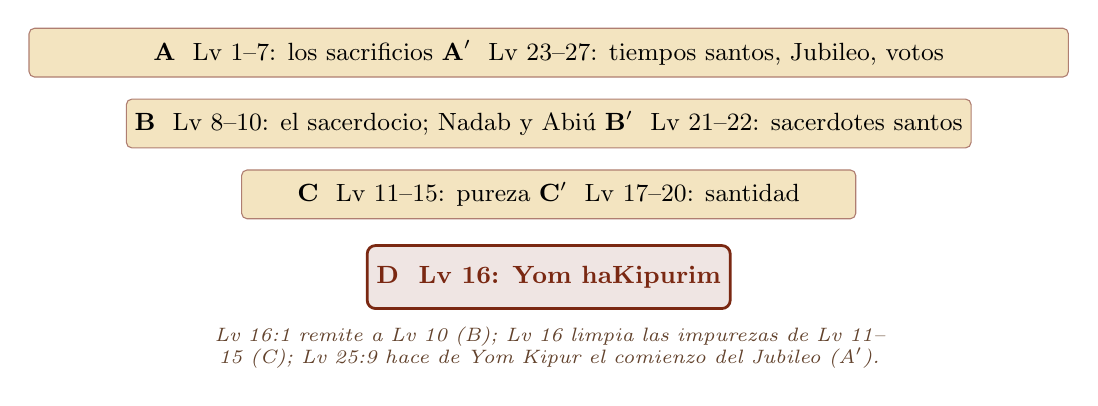
\begin{tikzpicture}[font=\small,x=1cm,y=1cm,
  bl/.style={draw=tierraroja!60,fill=papiro,rounded corners=2pt,minimum height=0.62cm,align=center,inner sep=3pt}]
 \node[bl,minimum width=13.2cm] (a) at (0,3.0) {\textbf{A} \ Lv 1--7: los sacrificios \hfill \textbf{A$'$} \ Lv 23--27: tiempos santos, Jubileo, votos};
 \node[bl,minimum width=10.4cm] (b) at (0,2.1) {\textbf{B} \ Lv 8--10: el sacerdocio; Nadab y Abiú \hfill \textbf{B$'$} \ Lv 21--22: sacerdotes santos};
 \node[bl,minimum width=7.8cm] (c) at (0,1.2) {\textbf{C} \ Lv 11--15: pureza \hfill \textbf{C$'$} \ Lv 17--20: santidad};
 \node[draw=tierraroja,line width=1pt,fill=tierraroja!12,rounded corners=3pt,minimum width=4.6cm,minimum height=0.8cm,align=center,font=\small\bfseries,text=tierraroja] (d) at (0,0.15) {D \ Lv 16: Yom haKipurim};
 \node[font=\scriptsize\itshape,text=sepia,text width=13cm,align=center] at (0,-0.75) {Lv 16:1 remite a Lv 10 (B); Lv 16 limpia las impurezas de Lv 11--15 (C); Lv 25:9 hace de Yom Kipur el comienzo del Jubileo (A$'$).};
\end{tikzpicture}\par
{\footnotesize\color{sepia}\textit{Figura 6.} Lv 16 en el centro del Levítico: una propuesta concéntrica simplificada. \textit{Nota.} Elaboración propia, inspirada en propuestas de varios autores (Douglas, 1999; Warning, 1999); los detalles se discuten.}
\end{center}

Las conexiones del capítulo con los bloques vecinos están en el texto y no dependen de la propuesta. Lv 16:1 remite a la muerte de Nadab y Abiú (Lv 10); las ``impurezas'' (\heb{טֻמְאֹת}, 16:16, 19) son las de Lv 11--15; y Lv 17 comienza con la prohibición de sacrificar a los ``demonios'' (\emph{se'irim}), palabra idéntica a la de los machos cabríos del capítulo anterior.

\subsection{El recorrido del sumo sacerdote: de dentro hacia fuera}
El rito tiene un movimiento espacial preciso. El sumo sacerdote entra desde el atrio hasta el lugar santísimo, y luego la sangre recorre el camino inverso: primero la \emph{kapóret}, después la tienda, finalmente el altar. Lo que se purifica va del centro a la periferia, del lugar más santo al menos santo, como quien limpia una casa empezando por la habitación interior; lo que se elimina, en cambio, sale del todo, fuera del campamento.

\begin{center}
\resizebox{\linewidth}{!}{%
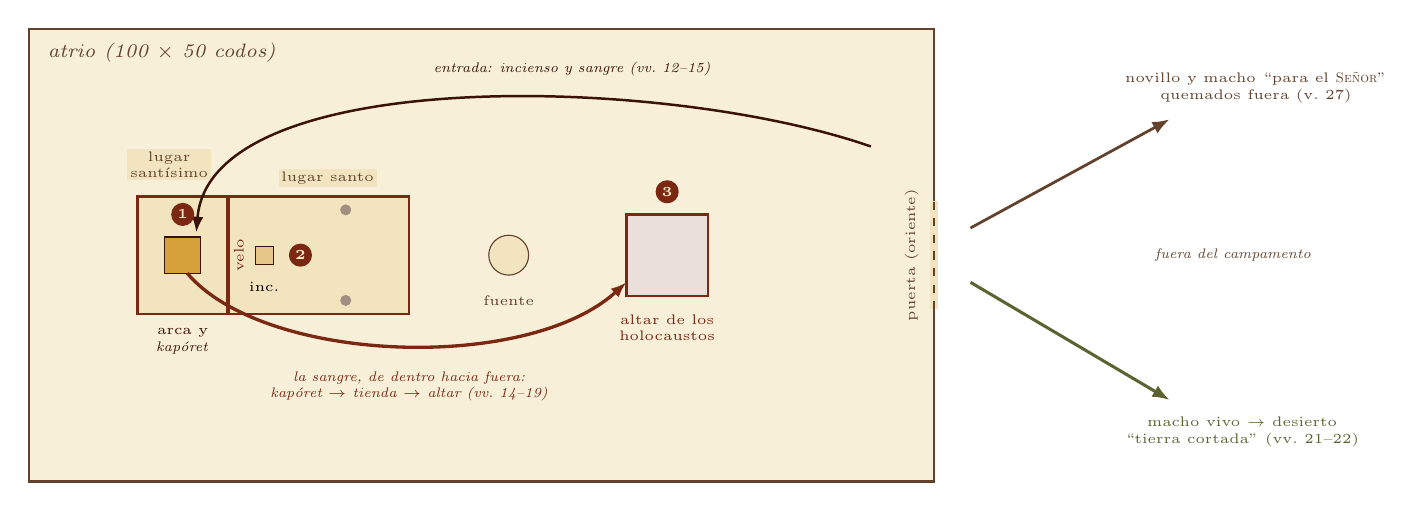
\begin{tikzpicture}[x=1.15cm,y=1.15cm,font=\scriptsize]
 % atrio
 \draw[sepia,line width=0.8pt,fill=papiro!60] (0,0) rectangle (10,5);
 \node[anchor=north west,text=sepia,font=\scriptsize\itshape] at (0.1,4.95) {atrio (100 $\times$ 50 codos)};
 % tienda
 \draw[tierraroja,line width=0.9pt,fill=papiro] (1.2,1.85) rectangle (4.2,3.15);
 \draw[tierraroja,line width=1.4pt] (2.2,1.85) -- (2.2,3.15);
 \node[text=tierraroja,font=\tiny,rotate=90] at (2.32,2.5) {velo};
 \node[text=sepia,font=\tiny,align=center,fill=papiro,inner sep=1pt] at (1.55,3.5) {lugar\\santísimo};
 \node[text=sepia,font=\tiny,align=center,fill=papiro,inner sep=1pt] at (3.3,3.35) {lugar santo};
 % arca
 \draw[fill=mostaza,draw=caferojizo] (1.5,2.3) rectangle (1.9,2.7);
 \node[font=\tiny,text=caferojizo,align=center] at (1.7,1.55) {arca y\\\emph{kapóret}};
 % incienso, candelero, mesa
 \draw[fill=mostaza!60,draw=caferojizo] (2.5,2.4) rectangle (2.7,2.6);
 \node[font=\tiny] at (2.6,2.15) {inc.};
 \fill[sepia!60] (3.5,2.0) circle (2pt); \fill[sepia!60] (3.5,3.0) circle (2pt);
 % fuente y altar
 \draw[sepia,fill=papiro] (5.3,2.5) circle (0.22);
 \node[font=\tiny,text=sepia] at (5.3,2.0) {fuente};
 \draw[tierraroja,fill=tierraroja!15,line width=0.8pt] (6.6,2.05) rectangle (7.5,2.95);
 \node[font=\tiny,text=tierraroja,align=center] at (7.05,1.7) {altar de los\\holocaustos};
 % puerta
 \draw[papiro,line width=3pt] (10,1.9) -- (10,3.1);
 \draw[sepia,line width=0.6pt,dashed] (10,1.9) -- (10,3.1);
 \node[font=\tiny,text=sepia,rotate=90] at (9.75,2.5) {puerta (oriente)};
 % entrada del sumo sacerdote
 \draw[-{Latex[length=2mm]},caferojizo,line width=0.9pt] (9.3,3.7) .. controls (7,4.5) and (2.0,4.6) .. (1.85,2.75);
 \node[font=\tiny\itshape,text=caferojizo] at (6.0,4.55) {entrada: incienso y sangre (vv.~12--15)};
 % sangre de dentro hacia fuera
 \draw[-{Latex[length=2mm]},tierraroja,line width=1.2pt] (1.75,2.3) .. controls (2.6,1.3) and (5.5,1.2) .. (6.6,2.2);
 \node[font=\tiny\itshape,text=tierraroja,align=center] at (4.2,1.05) {la sangre, de dentro hacia fuera:\\kapóret $\rightarrow$ tienda $\rightarrow$ altar (vv.~14--19)};
 % numeros
 \foreach \x/\y/\n in {1.7/2.95/1, 3.0/2.5/2, 7.05/3.2/3}{\node[circle,fill=tierraroja,text=papiro,font=\tiny\bfseries,inner sep=1.2pt] at (\x,\y) {\n};}
 % fuera
 \draw[-{Latex[length=2.2mm]},oliva,line width=1.1pt] (10.4,2.2) -- (12.6,0.9);
 \node[font=\tiny,text=oliva,align=center,anchor=west] at (12.0,0.55) {macho vivo $\rightarrow$ desierto\\``tierra cortada'' (vv.~21--22)};
 \draw[-{Latex[length=2.2mm]},sepia,line width=1pt] (10.4,2.8) -- (12.6,4.0);
 \node[font=\tiny,text=sepia,align=center,anchor=west] at (12.0,4.35) {novillo y macho ``para el \SENOR''\\quemados fuera (v.~27)};
 \node[font=\tiny\itshape,text=sepia] at (13.3,2.5) {fuera del campamento};
\end{tikzpicture}}\par
{\footnotesize\color{sepia}\textit{Figura 7.} Plano esquemático del tabernáculo y recorrido del día. \textit{Nota.} Elaboración propia sobre Éx 26--27; 30 y Lv 16; escala aproximada. 1 = \emph{kapóret} (1 + 7 aspersiones de cada sangre), 2 = tienda de reunión, 3 = altar (cuernos + 7 aspersiones).}
\end{center}

La sangre se aplica con una cuenta precisa: una vez ``hacia el propiciatorio al lado oriental'' y siete veces ``hacia el propiciatorio'' con la sangre del becerro (v. 14); lo mismo con la del macho cabrío (v. 15); y siete veces sobre el altar, después de untar sus cuernos (vv. 18--19). La Misná lo describe como una aspersión hacia arriba y siete hacia abajo (Misná Yomá 5:3--4). El número siete organiza también el vocabulario: la palabra \emph{kapóret} aparece siete veces en el capítulo y \emph{jatat}, catorce (conteos propios), y el rito ocurre en el mes séptimo. No conviene forzar la aritmética, pero la insistencia en el siete, número de la creación completa, presenta la purificación como total.

\subsection{Dos machos cabríos, un solo acto}
El versículo 5 fija el dato que gobierna todo lo demás: el pueblo entrega ``dos machos cabríos para expiación'', en singular, \heb{לְחַטָּאת}. Los dos animales forman una sola ofrenda con dos funciones (Milgrom, 1991; Wenham, 1979). Uno muere y su sangre purifica el santuario; el otro vive y se lleva las culpas confesadas. La suerte asigna las funciones, pero ambos son presentados ``delante de \SENOR''.

\begin{center}
\resizebox{\linewidth}{!}{%
\begin{tikzpicture}[font=\small,
  hd/.style={font=\scriptsize\bfseries,text=sepia},
  bx/.style={draw=tierraroja!65,fill=papiro,rounded corners=2pt,text width=3.55cm,align=center,inner sep=4pt,minimum height=1.25cm},
  fl/.style={-{Latex[length=2mm]},mostaza!80!tierraroja,line width=0.9pt}]
 \node[draw=tierraroja,line width=1pt,fill=tierraroja!10,rounded corners=3pt,text width=2.6cm,align=center,inner sep=5pt] (o) at (0,0) {Dos machos cabríos\\ \textbf{una} \emph{jatat}\\ \scriptsize (v.~5)};
 \node[hd] at (4.1,2.3) {Suerte}; \node[hd] at (8.2,2.3) {Destino}; \node[hd] at (12.3,2.3) {Sentido};
 \node[bx] (s1) at (4.1,1.1) {\heb{לַיהוָה}\\ ``para el \SENOR''\\ \scriptsize vv.~8--9};
 \node[bx] (d1) at (8.2,1.1) {degollado; su sangre ante y sobre la \emph{kapóret}\\ \scriptsize v.~15};
 \node[bx] (m1) at (12.3,1.1) {purga el santuario de impurezas, rebeliones y pecados\\ \scriptsize vv.~16--19};
 \node[bx] (s2) at (4.1,-1.1) {\heb{לַעֲזָאזֵל}\\ ``para Azazel''\\ \scriptsize vv.~8, 10};
 \node[bx] (d2) at (8.2,-1.1) {vivo; dos manos, confesión, envío al desierto\\ \scriptsize vv.~20--22};
 \node[bx] (m2) at (12.3,-1.1) {lleva las iniquidades ``a tierra cortada'', sin retorno\\ \scriptsize v.~22};
 \draw[fl] (o) -- (s1); \draw[fl] (o) -- (s2);
 \draw[fl] (s1) -- (d1); \draw[fl] (d1) -- (m1); \draw[fl] (s2) -- (d2); \draw[fl] (d2) -- (m2);
 \draw[decorate,decoration={brace,amplitude=6pt},sepia] (14.25,1.65) -- (14.25,-1.65) node[midway,right=7pt,font=\scriptsize,text width=1.6cm,align=left,text=sepia]{\emph{kipper}: un acto, dos movimientos (v.~30)};
\end{tikzpicture}}\par
{\footnotesize\color{sepia}\textit{Figura 8.} Los dos machos cabríos: suerte, destino y sentido. \textit{Nota.} Elaboración propia sobre Lv 16.}
\end{center}

En una de mis láminas señalé el paralelo más cercano, la purificación del leproso con dos avecillas (Lv 14:4--7). Una se degüella sobre agua corriente; la otra, mojada en la sangre de la primera, se suelta ``en el campo''. En la purificación de una casa contaminada, el mismo rito termina con una frase que ilumina Lv 16: ``Luego soltará la avecilla viva fuera de la ciudad sobre la faz del campo. Así hará expiación por la casa, y será limpia'' (Lv 14:53). También el animal que se suelta vivo ``hace expiación'' (\emph{kipper}); la purificación incluye la eliminación.

\subsection{Ecos intrabíblicos}
El lenguaje del día resuena en otros textos que la serie y la tradición cristiana leerán juntos.

\paragraph{Éxodo 32--34 y Números 14.} Las dos grandes rebeliones del desierto terminan con la fórmula de Éx 34:7: Dios ``perdona (\emph{nosé}) la iniquidad, la rebelión y el pecado'' (cf. Nm 14:18). Moisés intercede tras el becerro de oro con el verbo de Yom Kipur: ``quizá le aplacaré (\heb{אֲכַפְּרָה}) acerca de vuestro pecado'' (Éx 32:30). Tras el informe de los espías, Dios responde: ``Yo lo he perdonado conforme a tu dicho'' (Nm 14:20), pero la generación ``llevará'' sus iniquidades cuarenta años en el desierto (14:34). Perdón y juicio conviven, y el día en que las iniquidades son ``llevadas'' fuera del campamento es la imagen ritual de ese desenlace.

\paragraph{Isaías 53.} El Siervo ``fue cortado de la tierra de los vivientes'' (53:8), ``\SENOR{} cargó en él el pecado de todos nosotros'' (53:6) y ``habiendo él llevado el pecado de muchos'' (53:12). Los verbos de Lv 16:22 (\emph{nasá}, \emph{guezerá}) reaparecen aplicados a una persona.

\paragraph{Zacarías 3.} En una visión, el sumo sacerdote Josué está ``delante del ángel de \SENOR, y Satanás estaba a su mano derecha para acusarle'' (Zac 3:1). Dios reprende a Satanás, le quitan a Josué las vestiduras viles y le dicen: ``Mira que he quitado de ti tu pecado, y te he hecho vestir de ropas de gala'' (3:4); la visión termina con la promesa: ``quitaré el pecado de la tierra en un día'' (3:9). La escena reúne un sumo sacerdote, un cambio de vestiduras, un acusador reprendido y un pecado quitado ``en un día'', elementos todos de Yom Kipur, y da apoyo bíblico a quienes ven en el día una sentencia contra Satanás (véase §\ref{sec:azazel}).

\paragraph{Miqueas 7 y el Salmo 103.} ``Sepultará nuestras iniquidades, y echará en lo profundo del mar todos nuestros pecados'' (Mi 7:19); ``cuanto está lejos el oriente del occidente, hizo alejar de nosotros nuestras rebeliones'' (Sal 103:12). La poesía dice con imágenes de distancia lo que el macho vivo representa con un viaje.

\paragraph{Levítico 25 y el Jubileo.} El año cincuenta se anuncia en Yom Kipur: ``el día de la expiación haréis tocar la trompeta por toda vuestra tierra'' (Lv 25:9), y en él se ``pregona libertad'' (\heb{דְּרוֹר}, \emph{derór}, 25:10). El mismo día que limpia el santuario libera la tierra y a los esclavos. Isaías 61:1--2 retoma \emph{derór} (``a publicar libertad a los cautivos''), y es ese texto el que Jesús lee en Nazaret (Lc 4:18--19).

\begin{center}
\resizebox{\linewidth}{!}{%
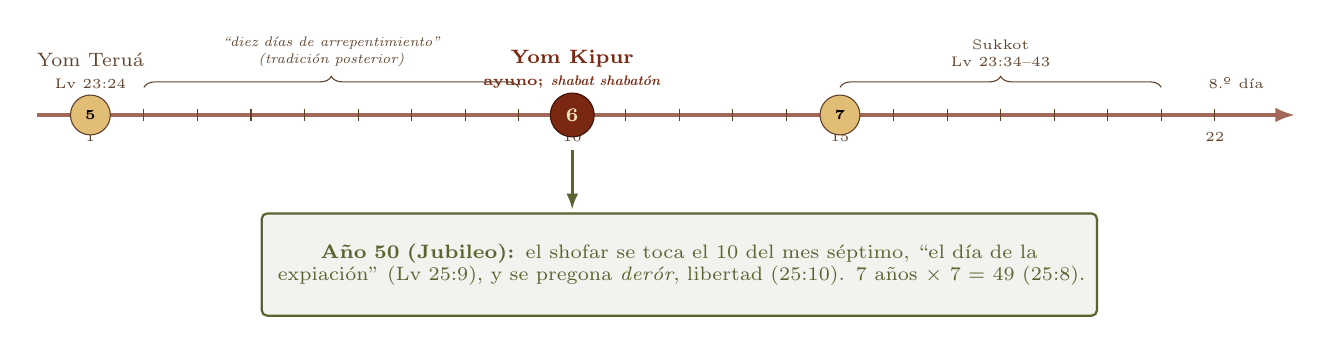
\begin{tikzpicture}[font=\scriptsize,x=0.68cm,y=1cm]
 \draw[line width=1.2pt,tierraroja!70,-{Latex[length=2.5mm]}] (0,0) -- (23.5,0);
 \foreach \d in {1,...,22}{\draw[sepia] (\d,-0.08) -- (\d,0.08);}
 \foreach \d in {1,10,15,22}{\node[below=3pt,font=\tiny,text=sepia] at (\d,0) {\d};}
 \node[circle,fill=mostaza!70,draw=sepia,minimum size=4.5mm,font=\tiny\bfseries] at (1,0) {5};
 \node[circle,fill=tierraroja,draw=caferojizo,minimum size=5.5mm,text=papiro,font=\scriptsize\bfseries] at (10,0) {6};
 \node[circle,fill=mostaza!70,draw=sepia,minimum size=4.5mm,font=\tiny\bfseries] at (15,0) {7};
 \node[above=6pt,text=sepia,align=center] at (1,0) {Yom Teruá\\ \tiny Lv 23:24};
 \node[above=6pt,text=tierraroja,font=\scriptsize\bfseries,align=center] at (10,0) {Yom Kipur\\ \tiny ayuno; \emph{shabat shabatón}};
 \draw[decorate,decoration={brace,amplitude=4pt},sepia] (2,0.35) -- (9,0.35) node[midway,above=4pt,font=\tiny\itshape,align=center]{``diez días de arrepentimiento''\\(tradición posterior)};
 \draw[decorate,decoration={brace,amplitude=4pt},sepia] (15,0.35) -- (21,0.35) node[midway,above=4pt,font=\tiny,align=center]{Sukkot\\ \tiny Lv 23:34--43};
 \node[above=6pt,text=sepia,align=center,font=\tiny] at (22.4,0) {8.º día};
 % jubileo
 \draw[oliva,line width=0.8pt,rounded corners=2pt,fill=oliva!8] (4.2,-1.25) rectangle (19.8,-2.55);
 \node[text=oliva,font=\scriptsize,align=center,text width=10.2cm] at (12,-1.9) {\textbf{Año 50 (Jubileo):} el shofar se toca el 10 del mes séptimo, ``el día de la expiación'' (Lv 25:9), y se pregona \emph{derór}, libertad (25:10). 7 años $\times$ 7 = 49 (25:8).};
 \draw[-{Latex[length=2mm]},oliva,line width=0.9pt] (10,-0.45) -- (10,-1.2);
\end{tikzpicture}}\par
{\footnotesize\color{sepia}\textit{Figura 9.} El mes séptimo: Teruá, Kipur y Sukkot, y el Jubileo anunciado en Yom Kipur. \textit{Nota.} Elaboración propia sobre Lv 23 y 25.}
\end{center}

%===================================================================
\section{Memorial, figura y esperanza: la lectura de la serie}\label{sec:serie}

El documento de referencia que enmarca esta serie (un curso de doctrina de la adoración de la línea sabatista de la Iglesia de Dios) dedica a la ``Solemnidad de las Expiaciones'' dos lecciones: la octava, que la sitúa en la historia de Israel, y la decimotercera, que la lee en el Nuevo Pacto. Expongo aquí su tesis con sus propios argumentos y añado al final las precisiones que el texto bíblico o la historia exigen.

\subsection{Una convocación perpetua dentro del Reglamento del Culto}
Para la serie, Levítico 23 es el ``Reglamento del Culto'', las convocaciones santas que Dios fijó ``en sus tiempos'' como ``estatuto perpetuo'', y lo distingue de ``la Ley de los sacrificios por el pecado'' (Lv 1--7; Nm 28--29), que Pablo llamaría ``la ley de los mandamientos expresados en ordenanzas'' (Ef 2:15; RV1909: ``en orden a ritos''), cumplida en el sacrificio de Cristo. La lección octava enumera cuatro rasgos de la Solemnidad de las Expiaciones en Lv 23: es una santa convocación el día 10 del mes séptimo; tiene el carácter de un sábado santo; es un día solemne de ayuno, porque ``afligiréis vuestras almas'' significa, según Sal 35:13 y 69:10, ``privarse de todo alimento de puesta de sol a puesta de sol''; y es un mandato perpetuo. Por eso la Iglesia la sigue guardando, y el documento cita como prueba que en la Iglesia apostólica ``el día del ayuno de la expiación era un hito importante'' (Hch 27:9).

\subsection{El memorial: el fin del juicio en el desierto}
Cada solemnidad, según la serie, conmemora un hito de la historia de Israel; la de las Expiaciones recuerda el fin del juicio de Dios sobre la nación en el desierto:

\begin{cita}[fontupper=\small\itshape]La entrada a la tierra de la promesa, ya era inminente, luego de la caída de los muros de Jericó; pasaba por el hecho ineludible de lograr el perdón de Dios; pues esta era la más explícita señal de que, por fin había concluido el juicio de Dios a la nación; y les había sido concedido el perdón, tras las rebeliones en el desierto; particularmente aquella en que se negaron a entrar en la Tierra Prometida, cuando regresaron los primeros doce espías enviados por Moisés.\fuente{(Documento de referencia, lección 8)}\end{cita}

La lección duodécima lo resume en un cuadro de correspondencias:

\begin{center}\small\renewcommand{\arraystretch}{1.18}
\begin{tabular}{@{}L{4.6cm}L{3.4cm}L{6.6cm}@{}}
\toprule
\textbf{Hito de Israel} & \textbf{Solemnidad} & \textbf{Nuevo Pacto} \\ \midrule
Israel salvado de la muerte & Pascua & Cristo nuestra Pascua (1~Co 5:7) \\
Israel libre del cautiverio & Ázimos & la Iglesia sin levadura (1~Co 5:8) \\
La entrega de la Ley & Pentecostés & el Espíritu derramado (Hch 2) \\
La toma de Jericó & Trompetas & el retorno de Cristo a la final trompeta (1~Co 15:52) \\
\textbf{Fin del juicio en el desierto} & \textbf{Expiación} & \textbf{fin del juicio a la casa de Dios (1~P 4:17); Satanás atado (Ap 20:1--3)} \\
Israel entra a Canaán & Cabañas & el Reino milenial \\
\bottomrule
\end{tabular}\par
{\footnotesize\color{sepia}\textit{Tabla 4.} La historia de Israel y el Reglamento del Culto según la serie. \textit{Nota.} Elaboración propia a partir de las lecciones 12 y 13 del documento de referencia.}
\end{center}

La secuencia del mes séptimo adquiere así un sentido histórico continuo. El toque de trompetas ante Jericó indicaba que había llegado el momento de la heredad; la expiación, que ``sus faltas habían sido purgadas'' y el juicio había concluido; las cabañas, que Israel se establecía en la tierra. ``La interrelación de estos tres hechos históricos, no es una casualidad'' (lección 12).

\subsection{La figura: el Sumo Pontífice y los dos machos cabríos}
La lección decimotercera comienza con el texto de 1~Jn 2:1--2 (``abogado tenemos para con el Padre, a Jesucristo el justo. Y él es la propiciación por nuestros pecados'') y explica por qué la Iglesia necesita un abogado: ``si decimos que no tenemos pecado, nos engañamos a nosotros mismos'' (1~Jn 1:8), y el juicio de Dios comienza por su casa (1~P 4:17). Recorre luego el ceremonial de Lv 16 en cuatro correspondencias:

\begin{enumerate}\setlength{\itemsep}{2pt}
\item \textbf{La presencia del Sumo Pontífice.} La expiación requería al sumo sacerdote; la Iglesia tiene ``tal sumo sacerdote, el cual se sentó a la diestra del trono de la Majestad en los cielos, ministro del santuario, y de aquel verdadero tabernáculo que levantó el Señor, y no el hombre'' (He 8:1--2), ``santo, inocente, sin mancha, apartado de los pecadores'' (He 7:26).
\item \textbf{El pecado cargado.} El sumo sacerdote expiaba los pecados que llevaba consigo; de Cristo se dice: ``Al que no conoció pecado, por nosotros lo hizo pecado, para que nosotros fuésemos hechos justicia de Dios en él'' (2~Co 5:21), porque ``\SENOR{} cargó en él el pecado de todos nosotros'' (Is 53:6).
\item \textbf{Los dos machos cabríos.} Uno ``se disponía para redimir la culpa ofreciendo su sangre''; el otro ``se identificaba con la causa de la culpa, por lo tanto era sacado del real''. Cristo, el Sumo Pontífice, cargó los pecados de la humanidad (1~Jn 2:2) y purificó el santuario celestial a su regreso a la diestra del Padre, ``cerrando para siempre la entrada de Satanás al solio de Dios'' (He 9:22--24).
\item \textbf{La salida del santuario.} ``Cuando el Sumo Pontífice salía del Lugar santísimo, el pueblo entendía que sus pecados habían sido expiados y que Dios había aceptado la sangre de los sacrificios. Cuando el Sumo Pontífice del Nuevo Pacto salga del Santuario Celestial, el Pueblo de Dios redimido por su sangre, sabrá que el juicio sobre ellos habrá concluido positivamente, ora estén durmiendo en el polvo de la tierra o aún vivan'' (lección 13).
\end{enumerate}

El juicio a la casa de Dios concluye, entonces, con el veredicto que se entrega a la Iglesia en la resurrección y la transformación: ``todos seremos transformados, en un momento, en un abrir y cerrar de ojos, a la final trompeta'' (1~Co 15:51--52), porque ``no se levantarán los malos en el juicio, ni los pecadores en la congregación de los justos'' (Sal 1:5). La vida eterna es ``dádiva de Dios'' (Ro 6:23), y ``se sabrá a quienes es otorgada al momento del retorno de nuestro Señor''.

\subsection{Azazel: el instigador que carga su culpa}
Lo más característico de la lectura de la serie es el macho cabrío para Azazel. El documento rechaza que represente a Cristo y argumenta desde Lv 16:26:

\begin{cita}[fontupper=\small\itshape]¿Por qué esta última ceremonia? Sin lugar a dudas para ser limpio de las inmundicias del pecado que significaba el contacto con éste macho cabrío, por esto quienes sostienen que este macho cabrío representa a Jesús están equivocados porque nunca nuestro Señor ni siquiera en el sepulcro fue contaminado.\fuente{(Documento de referencia, lección 13)}\end{cita}

El macho para Azazel figura a Satanás, ``el inductor de los pecados de la humanidad'', a quien un ángel ``con la llave del abismo, y una gran cadena en la mano'' prenderá y atará por mil años, ``para que no engañase más a las naciones'' (Ap 20:1--3). Que Satanás deba cargar con su parte lo explica la serie a partir de la forma en que Dios juzga en la Escritura:

\begin{itemize}\setlength{\itemsep}{2pt}
\item \textbf{Génesis 3.} Al dictar sentencia, Dios no juzga solo a Adán y Eva; el pecado tuvo un instigador, la serpiente, y ``él también debió comparecer y responder en la medida que participó en la rebelión del género humano''. La sentencia comienza por ella: ``Por cuanto esto hiciste, maldita serás entre todas las bestias\ldots{} Y pondré enemistad entre ti y la mujer, y entre tu simiente y la simiente suya; ésta te herirá en la cabeza, y tú le herirás en el calcañar'' (Gn 3:14--15). ``Esa es la forma que Dios enjuicia al Hombre''.
\item \textbf{1~Pedro 3:19 y Judas 6.} En el juicio de los días de Noé, detrás de la corrupción humana estuvieron ``los espíritus encarcelados'' (1~P 3:19), los ángeles que, según Judas, ``no guardaron su dignidad, sino que abandonaron su propia morada'' y que Dios ``ha guardado bajo oscuridad, en prisiones eternas, para el juicio del gran día'' (Jud 6). Para la serie, esas prisiones no son cárceles físicas sino la ``oscuridad'' que les impide alcanzar la sabiduría de Dios y obrar el bien.
\end{itemize}

Estos dos casos muestran, según el documento, ``la forma de actuar de Dios en sus juicios frente al pecado de la humanidad'': cuando juzga a los hombres, juzga también a quien los indujo. El folleto de la Iglesia de Dios Unida (2011), material del proyecto, desarrolla la misma lectura; el día tiene que ver ``no sólo con el perdón del pecado, sino que también representa la eliminación de la causa principal del pecado: Satanás y sus demonios''.

\subsection{La esperanza: del juicio al Reino}
La serie lee el mes séptimo como una secuencia escatológica. Trompetas anuncia el retorno de Cristo y la resurrección; Expiación, la conclusión del juicio a la Iglesia, la salida del Sumo Pontífice y el prendimiento de Satanás; Cabañas, el Reino milenial con sus santos; el octavo día, lo que sigue al Milenio. Así lo resume la lección decimocuarta: ``la salida de nuestro Sumo Pontífice del Lugar Santísimo en los cielos, determinará el fin del Juicio a la Iglesia, manifestado, en la Resurrección de los que duermen en Cristo y la Transformación de aquellos fieles que estén con vida\ldots{} y finalmente el prendimiento de Satanás''.

\subsection{Mis presentaciones anteriores: las fiestas, reloj de los tiempos proféticos}
En mis presentaciones sobre Yom Kipur (\emph{Yom Kippur B} y \emph{M}) desarrollé la misma línea escatológica con un recorrido propio: el pacto mosaico, los \emph{moadim}, Yom Kipur, el día de la ira, el Jubileo, el juicio y las sombras proféticas. El punto de partida era Lv 23:2: las fiestas son \heb{מוֹעֲדֵי יְהוָה} (\emph{moadé YHWH}, ``tiempos señalados del \SENOR'') que se proclaman como \heb{מִקְרָאֵי קֹדֶשׁ} (\emph{mikraé kódesh}). Recogí allí la glosa ``ensayo'' para \emph{mikrá} y concluí que las fiestas son ``el reloj de los tiempos proféticos'', sombra de lo por venir (Col 2:16--17).

El argumento léxico tiene una base real. La Septuaginta traduce \emph{moadim} con \grc{καιροί}: el sol y la luna son ``para señales, para las estaciones'' (\grc{εἰς καιρούς}, Gn 1:14), las fiestas se proclaman ``en sus tiempos'' (\grc{ἐν τοῖς καιροῖς αὐτῶν}, Lv 23:4; cf. Nm 9:3), y Dios ``hizo la luna para los tiempos'' (Sal 104:19 [103:19 LXX]). Pablo, que leía la Biblia griega, habla de ``los tiempos y las ocasiones'' (\grc{περὶ δὲ τῶν χρόνων καὶ τῶν καιρῶν}, 1~Ts 5:1) y de ``la dispensación del cumplimiento de los tiempos'' (\grc{τῶν καιρῶν}, Ef 1:10). De ahí inferí que el apóstol estructura los tiempos futuros según las fiestas.

\begin{nota}[Precisión]
\emph{Mikrá} viene de \heb{קָרָא} (``llamar, proclamar, leer''): significa ``convocación'' y, en Neh 8:8, ``lectura''. El sentido ``ensayo'' que aparece en algunas obras de divulgación (y en ciertas ediciones de la concordancia de Strong) es una analogía, no un significado hebreo atestiguado (Brown, Driver y Briggs, 1906; Koehler y Baumgartner, 2001). El vínculo \emph{moed} $\rightarrow$ \grc{καιρός} es real, pero \grc{καιρός} es palabra muy común; que en 1~Ts 5:1 o Ef 1:10 aluda a las fiestas es una inferencia posible, no un dato del texto. Mis láminas repiten también la leyenda de los setenta y dos traductores que, en celdas separadas, produjeron versiones idénticas: la narra la \emph{Carta de Aristeas} y la amplían Filón (\emph{Vida de Moisés} 2.37--40) y el Talmud (b. Meguilá 9a); es una leyenda sobre el origen de la Septuaginta, no un dato histórico.
\end{nota}

\subsection{El día del juicio y el día de la ira}
El centro de aquellas presentaciones es un cuadro que superpone dos escenas: el día del juicio, que es la Expiación de Lv 16, y el día de la ira de Dios, que anuncian los profetas y el Apocalipsis. Los profetas hablan de ``el día de su ira'' (Sal 110:5): ``Día de ira aquel día, día de angustia y de aprieto\ldots{} día de tiniebla y de oscuridad, día de nublado'' (Sof 1:15; cf. 1:7, 14--16; Is 13:9). El texto más cercano a Yom Kipur es Is 63:1--6, donde el guerrero que viene de Edom con las ropas rojas dice: ``He pisado yo solo el lagar\ldots{} y su sangre salpicó mis vestidos, y manché todas mis ropas. Porque el día de la venganza está en mi corazón, y el año de mis redimidos ha llegado'' (Is 63:3--4). Vinculé ``el año de mis redimidos'' (\heb{שְׁנַת גְּאוּלַי}, \emph{shenat gueulai}) con el Jubileo, que se anuncia en Yom Kipur (Lv 25:8--17), y con la figura del \emph{goel}, el pariente redentor que rescata la tierra y la persona (Lv 25:25; Rut 3--4), que también es vengador de la sangre (Nm 35) y que Job confiesa: ``Yo sé que mi Redentor (\heb{גֹּאֲלִי}) vive'' (Job 19:25; mis láminas dicen 9:25).

Los apóstoles retoman el lenguaje: el impenitente ``atesora\ldots{} ira para el día de la ira y de la revelación del justo juicio de Dios'' (Ro 2:5); el ángel arroja la vendimia ``en el gran lagar de la ira de Dios'' (Ap 14:19--20); y el que monta el caballo blanco ``estaba vestido de una ropa teñida en sangre'' (Ap 19:13). Un detalle del Apocalipsis recuerda con precisión Lv 16: ``el templo se llenó de humo por la gloria de Dios, y por su poder; y nadie podía entrar en el templo hasta que se hubiesen cumplido las siete plagas'' (Ap 15:8), como la nube de incienso que cubría la \emph{kapóret} (Lv 16:13) y como la regla de que ``ningún hombre estará en el tabernáculo'' mientras el sumo sacerdote expía (16:17). El refugio de los fieles está en el Salmo 27: ``él me esconderá en su tabernáculo en el día del mal'' (Sal 27:5).

\begin{center}
\resizebox{\linewidth}{!}{%
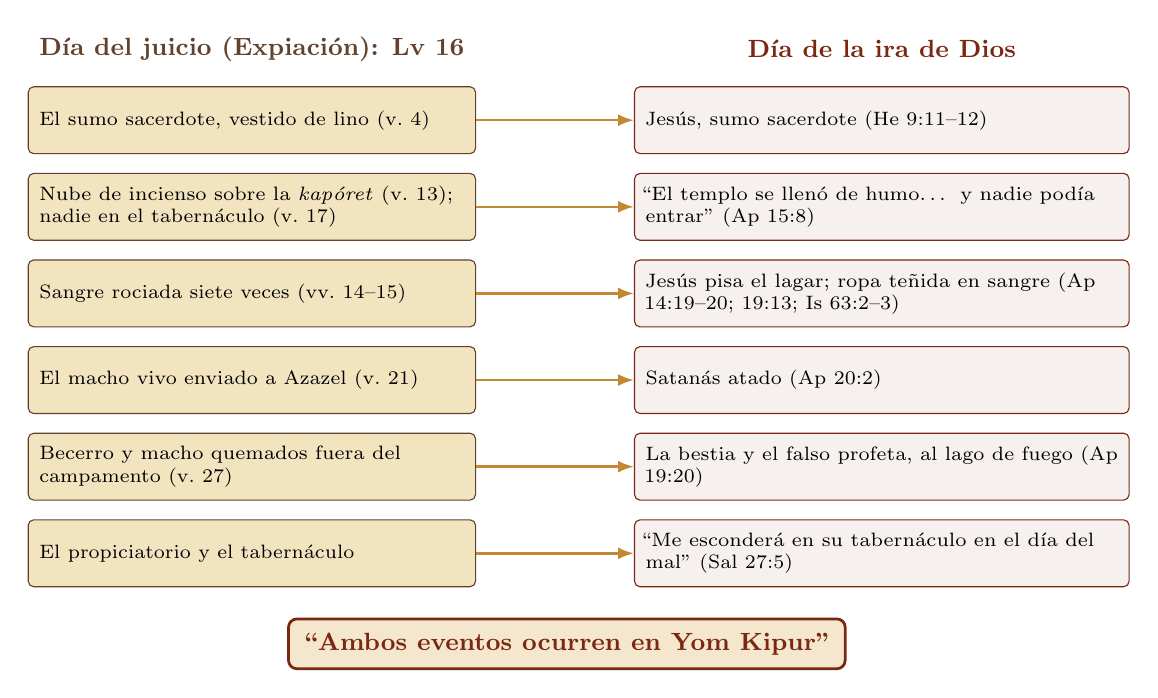
\begin{tikzpicture}[font=\scriptsize,
  l/.style={draw=sepia,fill=papiro,rounded corners=2pt,text width=5.4cm,align=left,inner sep=4pt,minimum height=0.85cm},
  r/.style={draw=tierraroja,fill=tierraroja!7,rounded corners=2pt,text width=6.0cm,align=left,inner sep=4pt,minimum height=0.85cm},
  fl/.style={-{Latex[length=2mm]},mostaza!80!tierraroja,line width=0.9pt}]
 \node[font=\small\bfseries,text=sepia] at (0,0.9) {Día del juicio (Expiación): Lv 16};
 \node[font=\small\bfseries,text=tierraroja] at (8,0.9) {Día de la ira de Dios};
 \foreach \y/\a/\b in {
   0/{El sumo sacerdote, vestido de lino (v.~4)}/{Jesús, sumo sacerdote (He 9:11--12)},
   -1.1/{Nube de incienso sobre la \emph{kapóret} (v.~13); nadie en el tabernáculo (v.~17)}/{``El templo se llenó de humo\ldots{} y nadie podía entrar'' (Ap 15:8)},
   -2.2/{Sangre rociada siete veces (vv.~14--15)}/{Jesús pisa el lagar; ropa teñida en sangre (Ap 14:19--20; 19:13; Is 63:2--3)},
   -3.3/{El macho vivo enviado a Azazel (v.~21)}/{Satanás atado (Ap 20:2)},
   -4.4/{Becerro y macho quemados fuera del campamento (v.~27)}/{La bestia y el falso profeta, al lago de fuego (Ap 19:20)},
   -5.5/{El propiciatorio y el tabernáculo}/{``Me esconderá en su tabernáculo en el día del mal'' (Sal 27:5)}}{
   \node[l] (a) at (0,\y) {\a}; \node[r] (b) at (8,\y) {\b}; \draw[fl] (a) -- (b);}
 \node[draw=tierraroja,line width=1pt,fill=mostaza!25,rounded corners=3pt,font=\small\bfseries,text=tierraroja,inner sep=5pt] at (4,-6.65) {``Ambos eventos ocurren en Yom Kipur''};
\end{tikzpicture}}\par
{\footnotesize\color{sepia}\textit{Figura 10.} El día del juicio (Expiación) y el día de la ira de Dios. \textit{Nota.} Elaboración propia a partir de mis presentaciones anteriores; lectura tipológica.}
\end{center}

\begin{nota}[Precisión]
El cuadro es una lectura tipológica mía: el Apocalipsis no menciona Yom Kipur ni fecha el día de la ira en el 10 del mes séptimo. Dos correspondencias piden cuidado. La del becerro y el macho quemados fuera del campamento con la bestia y el falso profeta difiere de la que hace Hebreos, que aplica esa misma quema a Jesús, que ``padeció fuera de la puerta'' (He 13:11--12); y en Ap 19:13 la sangre del vestido es, en el contexto de Is 63, la de los enemigos juzgados, no la del sacrificio. El paralelo entre Ap 15:8 y Lv 16:13, 17, en cambio, es estrecho, y la cercanía entre ``el año de mis redimidos'' (Is 63:4), el \emph{goel} y el Jubileo anunciado en Yom Kipur es un vínculo intrabíblico real. La tradición judía también une el día con el juicio, que se abre en Rosh haShaná y se sella en Yom Kipur (b. Rosh haShaná 16a--b).
\end{nota}

\subsection{Precisiones}
\begin{nota}[Precisión 1: tipología y calendario]
El vínculo entre Yom Kipur y el fin del juicio del desierto es lectura tipológica de la serie; el texto bíblico no lo establece. Hay apoyos temáticos reales: Nm 14 une perdón (``Yo lo he perdonado'', v. 20) y castigo (``llevaréis vuestras iniquidades cuarenta años'', v. 34), y en Guilgal Dios declara: ``Hoy he quitado de vosotros el oprobio de Egipto'' (Jos 5:9). Pero el calendario bíblico de la entrada a la tierra no coincide con el mes séptimo: Israel cruzó el Jordán ``el diez del mes primero'' (Jos 4:19), celebró la Pascua en Guilgal (Jos 5:10) y Jericó cayó después, en primavera. La correspondencia es de sentido y no de fecha.
\end{nota}

\begin{nota}[Precisión 2: otras lecturas memoriales antiguas]
La serie no es la primera en buscar un hecho histórico detrás del día. El libro de los Jubileos lo vincula con el cabrito degollado por los hijos de Jacob para engañar a su padre con la túnica de José (Jub 34:12--19). La tradición rabínica lo vincula con el perdón tras el becerro de oro: Moisés habría bajado con las segundas tablas el 10 del mes séptimo (Seder Olam Rabá 6; Rashi a Éx 33:11; cf. b. Taanit 30b). Las tres lecturas comparten la intuición de la serie: Yom Kipur conmemora un perdón después de una rebelión.
\end{nota}

\begin{nota}[Precisión 3: el argumento de Lv 16:26]
El argumento de la serie tiene una base textual: el que conduce el macho a Azazel debe lavar sus vestidos y su cuerpo antes de volver al campamento. Para exponerlo con justicia hay que añadir que Lv 16:28 impone el mismo lavado al que quema el becerro y el macho ``para el \SENOR'', cuya sangre entró en el lugar santísimo, y que en Nm 19:7--10 quedan impuros quienes preparan la vaca alazana, cuyas cenizas purifican. En la lógica del Levítico, lo que absorbe la impureza contamina a quien lo toca, sin que el animal mismo sea malo. El argumento más fuerte de la serie está en otro lugar, en el paralelo \heb{לַיהוָה} / \heb{לַעֲזָאזֵל} (v. 8), que presenta a Azazel como alguien opuesto al \SENOR, y en el hecho de que el macho vivo nunca se ofrece ni se sacrifica (véase §\ref{sec:azazel}).
\end{nota}

\begin{nota}[Precisión 4: Judas, 1~Enoc y Azazel]
Judas 6 tiene un trasfondo literario preciso: 1~Enoc 10:4--6 ordena atar a Azazel ``de pies y manos'', arrojarlo a las tinieblas en el desierto y cubrirlo de oscuridad ``hasta el gran día del juicio'' (trad. según Nickelsburg, 2001). Judas cita expresamente 1~Enoc en el v. 14 (1~En 1:9). El eco favorece la lectura de la serie, porque la imagen del ángel caído atado en la oscuridad del desierto hasta el juicio ya estaba asociada al nombre de Azazel en el judaísmo del siglo~\textsc{i}. En cuanto a 1~P 3:19, es uno de los textos más discutidos del Nuevo Testamento; una lectura extendida, cercana a la de la serie, entiende que Cristo proclamó su victoria a los ángeles rebeldes de Gn 6 (Dalton, 1989).
\end{nota}

\begin{nota}[Precisión 5: citas y vocabulario]
El texto de memoria de la lección 13 (``Mas ahora que habéis sido libertados del pecado\ldots{} la paga del pecado es muerte, mas la dádiva de Dios es vida eterna'') corresponde a Ro 6:22--23, no a 6:12--13. La alusión al ``ayuno de la expiación'' está en Hch 27:9 (el documento dice 28:9). El documento usa ``Sumo Pontífice'', voz de la Reina-Valera 1909 en Hebreos; la RVR1960 dice ``sumo sacerdote'' (\grc{ἀρχιερεύς}). Hebreos sostiene la idea de la serie de que el día trata los pecados de ignorancia: \grc{ἀγνοήματα} (He 9:7).
\end{nota}

\begin{nota}[Precisión 6: la autoría de Hebreos]
El documento de referencia atribuye Hebreos a Pablo (``el Apóstol Pablo declara''), como la tradición de Oriente desde el siglo~\textsc{ii}. La carta es anónima; ya Orígenes decía que ``quién escribió la epístola, solo Dios lo sabe'' (en Eusebio, \emph{Historia eclesiástica} 6.25.14), y los comentarios modernos la consideran obra de un autor del círculo paulino (Attridge, 1989; Lane, 1991). El argumento de la serie no depende de la autoría, pues Hebreos es Escritura canónica y su teología del sumo sacerdote tiene apoyo en cartas indiscutidas de Pablo (Ro 3:25; 8:34).
\end{nota}

%===================================================================
\section{La fiesta en Jesús y los apóstoles}\label{sec:mesias}

\subsection{El sumo sacerdote según el orden de Melquisedec}
La lectura cristiana de Yom Kipur pasa por una figura que Lv 16 no menciona, y que estudié desde Génesis en mi presentación \emph{Melk}. Al volver Abram de derrotar a Quedorlaomer, rey de Elam, y a sus aliados, le sale al encuentro en el valle del Rey ``Melquisedec, rey de Salem y sacerdote del Dios Altísimo'', que ``sacó pan y vino'', lo bendijo, y recibió de él ``los diezmos de todo'' (Gn 14:17--20). Es el primer \heb{כֹּהֵן} (\emph{kohen}, ``sacerdote'') de la Biblia, y su nombre, \heb{מַלְכִּי־צֶדֶק}, significa ``rey de justicia''; Salem, ``paz'' (He 7:2).

\begin{nota}[Precisión]
En esa presentación propuse que, como Elam era hijo de Sem (Gn 10:22), Abram habría dado muerte a un pariente, y que Melquisedec hace la paz con el pan y el vino. Es una hipótesis; el texto no explica el motivo del encuentro. Mis láminas leen también ``Noé, el octavo, pregonero de justicia'' (2~P 2:5, \grc{ὄγδοον Νῶε δικαιοσύνης κήρυκα}) como el octavo de una cadena de ``predicadores de justicia'' desde Adán (sin contar a Enoc, que fue llevado), continuada por Sem; la RVR1960 y la mayoría de los comentarios entienden que Dios ``guardó a Noé, pregonero de justicia, con otras siete personas'', es decir, las ocho personas del arca (cf. 1~P 3:20). La identificación de Melquisedec con Sem es una tradición judía antigua (Targum Neofiti y Pseudo-Jonatán a Gn 14:18; b. Nedarim 32b), no un dato del Génesis.
\end{nota}

El Salmo 110 da a la figura un lugar en la esperanza mesiánica. ``\SENOR{} dijo a mi Señor: Siéntate a mi diestra'' (v. 1) y ``Juró \SENOR, y no se arrepentirá: Tú eres sacerdote para siempre según el orden de Melquisedec'' (\heb{אַתָּה־כֹהֵן לְעוֹלָם עַל־דִּבְרָתִי מַלְכִּי־צֶדֶק}, v. 4). El rey davídico, que no era levita, recibe un sacerdocio de otro orden, anterior a Aarón y sin término.

\begin{nota}[Precisión textual]
Una de mis láminas afirma que el Texto Masorético ``ha sido alterado 134 veces''. La noticia procede de la tradición masorética, que enumera 134 lugares en que los escribas habrían escrito \heb{אֲדֹנָי} (\emph{Adonay}) donde se leía o escribía el tetragrama, por reverencia al Nombre (Ginsburg, 1897). Se trata de una tradición sobre la escritura del Nombre divino, y no prueba que se haya cambiado el sentido de un texto. En Sal 110:1 el hebreo distingue con claridad \heb{נְאֻם יְהוָה} (``dijo el \SENOR'') y \heb{לַאדֹנִי} (``a mi señor''), lectura que confirma la Septuaginta (\grc{εἶπεν ὁ κύριος τῷ κυρίῳ μου}) y que Jesús cita (Mt 22:44).
\end{nota}

Hebreos construye sobre el Salmo 110 su teología del sacerdocio de Cristo: ``Tú eres sacerdote para siempre, según el orden de Melquisedec'' (He 5:6). La palabra ``orden'' es \grc{τάξις}, ``orden, secuencia, turno'': Zacarías ofició ``según el orden de su clase'' (\grc{ἐν τῇ τάξει τῆς ἐφημερίας}, Lc 1:8), la de Abías, una de las veinticuatro clases sacerdotales que David estableció (1~Cr 24:3--10). Jesús entró ``hasta dentro del velo\ldots{} como precursor, hecho sumo sacerdote para siempre según el orden de Melquisedec'' (He 6:19--20). Melquisedec, ``sin padre, sin madre, sin genealogía'', fue ``hecho semejante al Hijo de Dios'' y ``permanece sacerdote para siempre'' (He 7:3); el silencio de Génesis sobre su origen se lee como figura de un sacerdocio que se constituye ``según el poder de una vida indestructible'' (He 7:16) y que se funda en un juramento (He 7:20--28). La justicia (\heb{צֶדֶק}, \emph{tsédeq}; \grc{δικαιοσύνη}) une el nombre del rey-sacerdote, la línea sacerdotal de Sadoc (2~S 8:17) y al Mesías ``justo'' (1~Jn 2:1, 29).

En mis láminas tracé en los evangelios una ``transferencia del orden''. Juan el Bautista, de linaje sacerdotal (Lc 1:5), bautiza a Jesús, que dice: ``así conviene que cumplamos toda justicia'' (Mt 3:15). En el juicio ante el sanedrín, Caifás ``rasgó sus vestiduras'' (Mt 26:65), gesto que la Ley prohibía al sumo sacerdote (Lv 10:6; 21:10); la túnica de Jesús, en cambio, ``era sin costura, de un solo tejido de arriba abajo'' (Jn 19:23), y no se rasgó. La Iglesia participa de ese sacerdocio, pues Cristo ``nos hizo reyes y sacerdotes para Dios'' (Ap 1:6; 5:10).

\begin{nota}[Precisión]
La ``transferencia del orden'' es una lectura tipológica mía. El contraste entre las vestiduras de Caifás y la túnica sin costura es sugerente; Josefo describe el manto del sumo sacerdote como tejido de una sola pieza (\emph{Ant.} 3.161), lo que ha llevado a varios intérpretes a ver en Jn 19:23 una alusión sacerdotal, pero Juan cita expresamente el Salmo 22 como clave de la escena (Jn 19:24).
\end{nota}

El judaísmo del Segundo Templo desarrolló la figura de un modo que toca de lleno el día de las expiaciones. El documento de Qumrán llamado 11QMelquisedec (11Q13) combina Lv 25 (el Jubileo), Dt 15:2 (la remisión) e Is 61:1 (``a publicar libertad a los cautivos'') y anuncia que Melquisedec ``les proclamará la liberación'' para librarlos de sus iniquidades; eso ocurrirá en el décimo jubileo, ``y el día de las expiaciones es el final del décimo jubileo, en el que se hará expiación por todos los hijos de la luz''. Reescribe además Is 61:2 como ``el año del favor de Melquisedec'' y lo presenta ejecutando el juicio de Dios contra Belial y los espíritus de su lote (11Q13 II 4--13; trad. según García Martínez, 1992, con lagunas reconstruidas).

\begin{nota}[Precisión]
11QMelquisedec es un texto fragmentario del siglo~\textsc{i} a.\,e.\,c., y varias palabras clave (entre ellas ``expiaciones'' en la línea 7) están reconstruidas por los editores. Aun así, la combinación de Jubileo, Yom Kipur, liberación de las iniquidades y juicio contra Belial está bien atestiguada (Bergsma, 2007), y ofrece un paralelo antiguo a dos ideas de la serie y de mis láminas: el día de las expiaciones como acontecimiento escatológico y como juicio contra el adversario.
\end{nota}

\subsection{Hebreos 9: el Yom Kipur del Mesías}
Hebreos 9 es la exposición más extensa de Yom Kipur en el Nuevo Testamento: el autor describe primero el tabernáculo y su ritual (9:1--10) y luego lee la obra de Cristo con las categorías del día (9:11--28).

\begin{cita}Pero estando ya presente Cristo, sumo sacerdote de los bienes venideros, por el más amplio y más perfecto tabernáculo, no hecho de manos, es decir, no de esta creación, y no por sangre de machos cabríos ni de becerros, sino por su propia sangre, entró una vez para siempre en el Lugar Santísimo, habiendo obtenido eterna redención.\fuente{(He 9:11--12)}\end{cita}

\begin{cita}Porque no entró Cristo en el santuario hecho de mano, figura del verdadero, sino en el cielo mismo para presentarse ahora por nosotros ante Dios\ldots{} así también Cristo fue ofrecido una sola vez para llevar los pecados de muchos; y aparecerá por segunda vez, sin relación con el pecado, para salvar a los que le esperan.\fuente{(He 9:24, 28)}\end{cita}

\begin{center}\small\renewcommand{\arraystretch}{1.22}
\begin{tabular}{@{}L{5.4cm}L{5.4cm}L{3.8cm}@{}}
\toprule
\textbf{Levítico 16} & \textbf{Hebreos} & \textbf{Contraste} \\ \midrule
Aarón, sumo sacerdote pecador, ofrece primero por sí (vv. 6, 11) & Cristo ``no tiene necesidad\ldots{} de ofrecer primero sacrificios por sus propios pecados'' (7:27) & sin pecado propio \\
``una vez al año'' (v. 34) & ``una vez para siempre'' (\grc{ἐφάπαξ}, 9:12; 10:10) & una vez, no cada año \\
sangre de becerro y machos cabríos (vv. 14--15) & ``por su propia sangre'' (9:12); ``la sangre de los toros y de los machos cabríos no puede quitar los pecados'' (10:4) & sangre propia \\
tabernáculo terrenal; la \emph{kapóret} tras el velo (v. 2) & ``el cielo mismo\ldots{} ante Dios'' (9:24) & santuario celestial \\
se purifican el santuario, la tienda y el altar (vv. 16--20) & ``las cosas celestiales mismas, con mejores sacrificios'' (9:23) & purificación celestial \\
el macho lleva las iniquidades (v. 22) & ``para llevar (\grc{ἀνενεγκεῖν}) los pecados de muchos'' (9:28; Is 53:12) & lleva el pecado \\
nadie en la tienda hasta que salga (v. 17) & ``aparecerá por segunda vez\ldots{} para salvar a los que le esperan'' (9:28) & la salida esperada \\
los cuerpos quemados fuera del campamento (v. 27) & ``Jesús\ldots{} padeció fuera de la puerta. Salgamos, pues, a él, fuera del campamento'' (13:11--13) & fuera del campamento \\
el velo cierra el acceso (v. 2; He 9:8) & ``camino nuevo y vivo\ldots{} a través del velo, esto es, de su carne'' (10:20) & acceso abierto \\
\bottomrule
\end{tabular}\par
{\footnotesize\color{sepia}\textit{Tabla 5.} Levítico 16 y Hebreos: correspondencias. \textit{Nota.} Elaboración propia; textos de la RVR1960.}
\end{center}

Tres rasgos de la lectura de Hebreos piden un comentario.

\paragraph{La purificación del santuario celestial.} ``Fue, pues, necesario que las figuras de las cosas celestiales fuesen purificadas así; pero las cosas celestiales mismas, con mejores sacrificios que estos'' (He 9:23). El autor aplica al cielo la lógica de Lv 16:16, según la cual el santuario se purifica. Los comentaristas discuten qué significa que lo celestial necesite purificación: la inauguración del nuevo santuario, la limpieza de la conciencia de los adoradores o la eliminación del pecado del ámbito de la presencia de Dios (Attridge, 1989; Lane, 1991). La serie lee aquí que Cristo cerró ``para siempre la entrada de Satanás al solio de Dios'', idea que encuentra apoyo en Ap 12:7--10, donde el acusador es arrojado del cielo.

\paragraph{La salida del sumo sacerdote.} He 9:28 tiene la estructura del día. Mientras el sumo sacerdote estaba dentro, el pueblo esperaba en el atrio, y su salida era la señal de que la expiación había sido aceptada (Lv 16:17--18, 24; cf. Si 50:5). Cristo ``aparecerá por segunda vez'' (\grc{ἐκ δευτέρου\ldots{} ὀφθήσεται}) a ``los que le esperan'' (\grc{τοῖς αὐτὸν ἀπεκδεχομένοις}). Hebreos describe así la segunda venida con la liturgia de Yom Kipur, y la Iglesia queda situada entre la entrada y la salida de su sumo sacerdote. Es la base neotestamentaria más clara de lo que la serie llama la ``salida del Sumo Pontífice''.

\paragraph{Una vez para siempre.} Hebreos subraya lo que Yom Kipur no podía hacer: ``en estos sacrificios cada año se hace memoria de los pecados'' (He 10:3), mientras que Cristo, ``habiendo ofrecido una vez para siempre un solo sacrificio por los pecados, se ha sentado a la diestra de Dios'' (10:12). El sumo sacerdote de Levítico nunca se sentaba en el santuario; que Cristo se siente es señal de obra terminada.

\begin{nota}[Precisión: Hebreos y la vigencia del día]
Hebreos trata el sacrificio, no la observancia del 10 de Tishri por los creyentes. De ``una vez para siempre'' se ha deducido que el día perdió su sentido, y de Col 2:16--17 (``sombra de lo que ha de venir'') que la sombra sigue señalando lo que aún vendrá. La serie sostiene esta segunda lectura y apoya la observancia en Hch 27:9 y en el carácter ``perpetuo'' del estatuto (Lv 16:29; 23:31). El debate excede este capítulo; basta aquí con anotar que Hebreos describe la entrada y la segunda aparición del sumo sacerdote como acontecimientos distintos, y que la segunda está todavía por cumplirse.
\end{nota}

\subsection{El velo rasgado}
En la muerte de Jesús, ``el velo del templo se rasgó en dos, de arriba abajo'' (Mt 27:51; cf. Mc 15:38; Lc 23:45). El \grc{καταπέτασμα} es, en la Septuaginta, el nombre del velo interior que separaba el lugar santísimo (Éx 26:31--33; Lv 16:2). Hebreos da la clave teológica: ``teniendo libertad para entrar en el Lugar Santísimo por la sangre de Jesucristo, por el camino nuevo y vivo que él nos abrió a través del velo, esto es, de su carne'' (He 10:19--20). Lo que en Lv 16 estaba reservado a un hombre, un día y bajo amenaza de muerte, queda abierto para el pueblo: ``acerquémonos, pues, confiadamente al trono de la gracia'' (He 4:16). En mis láminas lo resumí en una frase: ``Hoy con Yeshúa tenemos entrada al Lugar Santísimo''.

\subsection{Pablo y Juan}
\paragraph{Romanos 3:25.} El sentido de \grc{ἱλαστήριον} ya se discutió (§4). Si Pablo alude a la \emph{kapóret}, su argumento es que Dios ``puso'' públicamente a Cristo como el lugar de la expiación, para ``manifestar su justicia'' respecto de los pecados pasados que había soportado en su paciencia; lo que Yom Kipur hacía año tras año, oculto tras el velo, queda resuelto y expuesto en la cruz.

\paragraph{2~Corintios 5:21.} ``Al que no conoció pecado, por nosotros lo hizo pecado''. Como en hebreo \emph{jatat} significa ``pecado'' y ``sacrificio por el pecado'', y la Septuaginta usa a veces \grc{ἁμαρτία} para el sacrificio (Lv 4:21, 24), algunos intérpretes traducen ``lo hizo sacrificio por el pecado''; otros mantienen el sentido directo de un intercambio. En ambos casos el lenguaje viene del sistema que culmina en Lv 16.

\paragraph{1~Juan 1:8 -- 2:2.} Es el texto con que la serie abre la lección 13. Juan une la confesión (``Si confesamos nuestros pecados, él es fiel y justo para perdonar'', 1:9), el abogado ante el Padre (2:1) y la propiciación universal: ``él es la propiciación (\grc{ἱλασμός}) por nuestros pecados; y no solamente por los nuestros, sino también por los de todo el mundo'' (2:2). La confesión del pueblo sobre el macho vivo (Lv 16:21) y la intercesión del sumo sacerdote encuentran aquí su forma cristiana.

\subsection{Hechos 27:9: ``el ayuno''}
Lucas fecha el peligro de la navegación ``por haber pasado ya el ayuno'' (Hch 27:9). La expresión \grc{ἡ νηστεία} con artículo designa un ayuno conocido por todos, y la mayoría de los comentarios la identifica con Yom Kipur, que Filón y Josefo llaman del mismo modo. El texto prueba que el día seguía siendo una referencia de calendario para Lucas y su círculo décadas después de la resurrección; la serie lo interpreta, además, como indicio de que la Iglesia apostólica lo guardaba.

\subsection{El Apocalipsis}
Varios cuadros del Apocalipsis usan el mobiliario de Yom Kipur. Un ángel ``con un incensario de oro'' ofrece incienso con las oraciones de los santos ``sobre el altar de oro que estaba delante del trono'' (Ap 8:3--4). Al sonar la séptima trompeta, ``el templo de Dios fue abierto en el cielo, y el arca de su pacto se veía en el templo'' (Ap 11:19); lo que solo el sumo sacerdote veía una vez al año, entre nubes de incienso, queda a la vista. Y en Ap 20:1--3 el dragón, ``la serpiente antigua, que es el diablo y Satanás'', es atado, arrojado al abismo y sellado ``para que no engañase más a las naciones''. La serie une este último texto con el macho para Azazel; el paralelo más cercano en la literatura judía es 1~Enoc 10:4--6, donde Azazel es atado y arrojado a la oscuridad hasta el día del juicio.

\subsection{Ecos en los evangelios}
En mis presentaciones recogí otros ecos que la tradición cristiana ha visto en la pasión:
\begin{itemize}\setlength{\itemsep}{2pt}
\item \textbf{Las suertes.} ``Repartieron entre sí mis vestidos, y sobre mi ropa echaron suertes'' (Sal 22:18 [22:19]; Mc 15:24; Jn 19:24). Juan cita el salmo de manera explícita; la conexión con las suertes de Lv 16:8 es un eco posible y no un cumplimiento declarado.
\item \textbf{Barrabás.} Pilato ``les soltó a Barrabás, y entregó a Jesús\ldots{} para que fuese crucificado'' (Mc 15:15). Orígenes ya vio en el preso liberado una figura del macho enviado al desierto (\emph{Homilías sobre Levítico} 10.2), lectura que se ha repetido desde entonces (Stökl Ben Ezra, 2003).
\item \textbf{La escarlata.} Los soldados le echaron ``un manto de escarlata'' (Mt 27:28). La \emph{Epístola de Bernabé} (ca. 100--130 e.\,c.) relaciona la lana escarlata atada al macho cabrío con el manto escarlata de Cristo en su venida (Bernabé 7:6--11; Holmes, 2007).
\item \textbf{Fuera del campamento.} ``Jesús, para santificar al pueblo mediante su propia sangre, padeció fuera de la puerta'' (He 13:12), como los cuerpos del becerro y del macho cabrío quemados fuera del campamento (Lv 16:27).
\item \textbf{El sacerdote que bendice.} Al despedirse, Jesús ``alzando sus manos, los bendijo'' y ``fue llevado arriba al cielo'' (Lc 24:50--51), gesto que recuerda a Aarón cuando ``alzó\ldots{} sus manos hacia el pueblo y lo bendijo'' (Lv 9:22) y al sumo sacerdote Simón en Si 50:20 (eco posible).
\end{itemize}

%===================================================================
\section{La fiesta en la tradición judía}\label{sec:tradicion}

Lo que sigue es tradición rabínica y litúrgica, valiosa para conocer cómo vivió Israel el día, pero posterior al texto bíblico y, en parte, a la destrucción del templo.

\subsection{El servicio del Segundo Templo según la Misná}
El tratado \emph{Yomá} reconstruye el día con una minuciosidad que me impresionó cuando preparé las láminas de esta fiesta, que incluyen numerosas escenas de ese servicio (la preparación, las inmersiones, la caja de las suertes, el incienso, la sangre, el puente hacia el desierto):
\begin{itemize}\setlength{\itemsep}{2pt}
\item \textbf{Siete días de separación.} El sumo sacerdote dejaba su casa siete días antes y se preparaba leyendo y practicando el rito (Misná Yomá 1:1--3), a imitación de los siete días de la consagración de Aarón (Lv 8:33). Los ancianos le hacían jurar que no cambiaría nada de lo enseñado (1:5), en alusión a la disputa con los saduceos sobre el momento de poner el incienso.
\item \textbf{Tres confesiones.} Con las manos sobre el becerro, confesaba por sí y su casa (3:8); luego por sí, su casa y los sacerdotes (4:2); y sobre el macho vivo, por todo Israel (6:2). La fórmula era: ``Te suplico, oh \SENOR: he cometido iniquidad, me he rebelado y he pecado delante de ti, yo y mi casa\ldots{}, como está escrito en la Torá de Moisés tu siervo: porque en este día se hará expiación por vosotros'' (3:8, trad. propia según Danby, 1933). Cada confesión citaba así Lv 16:30 y pronunciaba el Nombre. Al oírlo, sacerdotes y pueblo se postraban y respondían: ``Bendito sea el nombre de la gloria de su reino por siempre jamás'' (6:2). Según una \emph{baraita} del Talmud, el sumo sacerdote pronunciaba el Nombre diez veces en el día: tres en cada una de las tres confesiones y una al echar las suertes (b. Yomá 39b).
\item \textbf{La caja de las suertes.} Las dos suertes, de madera y luego de oro, se sacaban de una urna; el sumo sacerdote decía ``Para el \SENOR, una ofrenda por el pecado'' (3:9; 4:1).
\item \textbf{La cinta escarlata.} Se ataba una cinta de lana escarlata a la cabeza del macho para Azazel (4:2). En el despeñadero, el encargado partía la cinta, ataba una mitad a una roca y otra entre los cuernos, y empujaba al animal hacia atrás (6:6). Según Rabí Ismael, había otra cinta en la puerta del santuario que se volvía blanca, en cumplimiento de Is 1:18: ``si vuestros pecados fueren como la grana, como la nieve serán emblanquecidos'' (6:8).
\item \textbf{El camino al desierto.} Una rampa salía del templo; había diez puestos con comida y agua a lo largo del camino, y unos ``babilonios'' tiraban del pelo del animal gritando: ``¡Toma y vete!'' (6:4--5).
\item \textbf{La lectura y la oración.} El sumo sacerdote leía en voz alta Lv 16 y 23:26--32, y recitaba de memoria Nm 29:7--11 (7:1). En el lugar santísimo hacía una oración breve, ``para no atemorizar a Israel'' (5:1). Al terminar, el pueblo lo acompañaba a su casa y él celebraba una fiesta ``porque había salido en paz del santuario'' (7:4).
\end{itemize}

\begin{nota}[Precisión: ¿Misná o Talmud?]
En mis láminas atribuí a la Misná la noticia de que la cinta dejó de blanquearse cuarenta años antes de la destrucción, y no corresponde. La Misná solo describe el blanqueamiento (Yomá 6:8); los cuarenta años aparecen en una \emph{baraita} del Talmud de Babilonia (b. Yomá 39b; cf. Talmud de Jerusalén, Yomá 6:3), junto con otros tres signos: la suerte ``para el \SENOR'' no salió en la mano derecha, la lámpara occidental del candelero se apagaba y las puertas del santuario se abrían solas. Se trata de tradición rabínica tardía; relacionarla con la muerte de Jesús es una lectura cristiana.
\end{nota}

\subsection{Del templo a la sinagoga}
Después del año 70, el día se reorganizó en torno a la oración. La Misná ya afirma que ``la muerte y el día de las expiaciones expían con el arrepentimiento'' (Yomá 8:8) y fija un principio ético decisivo: ``las transgresiones entre el hombre y Dios, el día de las expiaciones las expía; las transgresiones entre el hombre y su prójimo, el día de las expiaciones no las expía hasta que haya apaciguado a su prójimo'' (8:9). Rabí Aquiba cierra el tratado con una imagen: así como el baño ritual purifica a los impuros, ``el Santo, bendito sea, purifica a Israel'' (8:9).

La liturgia posterior añadió elementos que también recogí en las láminas:
\begin{itemize}\setlength{\itemsep}{2pt}
\item \textbf{Los diez días de arrepentimiento} entre Rosh haShaná y Yom Kipur, y la imagen de los libros abiertos, en que los justos son inscritos para la vida y la sentencia de los intermedios queda suspendida hasta Yom Kipur (b. Rosh haShaná 16a--b).
\item \textbf{El \emph{Avodá}}, la recitación poética del servicio del sumo sacerdote en la oración adicional (\emph{musaf}), en la que la congregación se postra al recordar el Nombre.
\item \textbf{Las lecturas}: Lv 16 en la mañana; Is 57:14 -- 58:14 como lectura profética, con su crítica del ayuno sin justicia (``¿No es más bien el ayuno que yo escogí, desatar las ligaduras de impiedad\ldots?'', Is 58:6); y el libro de Jonás en la tarde (b. Meguilá 31a), con su mensaje de arrepentimiento y misericordia para Nínive.
\item \textbf{La \emph{Neilá}}, ``cierre'', la oración final al ponerse el sol; el nombre recuerda el cierre de las puertas del templo (Misná Taanit 4:1). El toque de shofar al final del día es costumbre posterior, distinta del shofar del Jubileo de Lv 25:9.
\item \textbf{\emph{Kol Nidré}} (``todos los votos''), fórmula aramea de anulación de votos al comienzo del día, documentada en la época de los gueonim (s.~\textsc{viii}--\textsc{ix}); y \emph{kaparot}, costumbre medieval de girar un ave sobre la cabeza, combatida por varios rabinos.
\end{itemize}

\begin{nota}[Precisión: el ``gran shofar'']
La idea de tres trompetas (la ``primera'' en Shavuot, la ``última'' en Rosh haShaná y la ``gran trompeta'' en Yom Kipur) que aparece en algunas láminas pertenece a la enseñanza mesiánica popular, no a la Biblia ni a la Misná. Lo bíblico es que el shofar del Jubileo suena en Yom Kipur (Lv 25:9) y que los profetas anuncian una ``gran trompeta'' para la reunión de los dispersos (Is 27:13; cf. Mt 24:31). La asociación de ese texto con Yom Kipur es interpretativa.
\end{nota}

%===================================================================
\section{Discusión de interpretaciones}

\subsection{¿Qué purifica el día?}
Todos los intérpretes aceptan que Yom Kipur purifica el santuario y, por medio de él, al pueblo (Lv 16:16, 30). La discusión está en el mecanismo. Para Milgrom (1991), el pecado y la impureza del pueblo contaminan el santuario a distancia, en grados: las faltas inadvertidas manchan el altar exterior, las graves del pueblo llegan al lugar santo, y las rebeliones deliberadas (\emph{peshaím}) penetran hasta la \emph{kapóret}; Yom Kipur limpia todas las zonas, y el macho vivo se lleva las rebeliones, que no tenían sacrificio. Levine (1989) acentúa el sentido de ``borrar'' la contaminación con la sangre. Gane (2005) sostiene que la \emph{jatat} ordinaria purifica al oferente durante el año y que en Yom Kipur Dios purga su propia morada de las faltas ya perdonadas, en lo que llama un juicio que vindica la justicia de Dios al perdonar. Wenham (1979) y Hartley (1992) subrayan que la purificación es a la vez cultual y moral: el pueblo confiesa sus pecados y ``afligirá su alma''.

La lectura de Gane nace de la exégesis de Levítico y, aun así, se acerca a la de la serie: el día concluye un proceso en lugar de inaugurar el perdón, y lo que se cierra es la cuenta de los pecados ya perdonados. La serie proyecta ese cierre a la segunda venida de Cristo.

\subsection{¿Quién o qué es Azazel?}\label{sec:azazel}
Ninguna pregunta del capítulo ha recibido tantas respuestas. La tabla reúne las principales, con sus fuentes y sus dificultades.

\begin{center}\small\renewcommand{\arraystretch}{1.2}
\begin{tabular}{@{}L{2.9cm}L{4.6cm}L{3.8cm}L{3.5cm}@{}}
\toprule
\textbf{Lectura} & \textbf{Argumento principal} & \textbf{Fuentes y autores} & \textbf{Dificultad} \\ \midrule
El macho que se va & etimología \emph{ez ozel}; el animal ``enviado'' & Septuaginta; Símaco; Vulgata; Tyndale & ``enviarlo \emph{a} Azazel'' (v. 10) \\
Un lugar escarpado & destino geográfico del animal & Misná Yomá 6; b. Yomá 67b; Targum Ps.-Jonatán; Driver (1956) & el texto ya dice ``al desierto'' \\
Remoción total & nombre abstracto & Brown, Driver y Briggs (1906) & raíz poco atestiguada \\
Un ser demoníaco del desierto & paralelo \emph{laYHWH} / \emph{laAzazel}; los \emph{se'irim} de Lv 17:7 & 1~Enoc 8; 10; Milgrom (1991); Levine (1989); Hartley (1992); Wright (1987) & no se le ofrece nada; el rito es ``delante de \SENOR'' \\
Satanás, el instigador, que recibe la culpa que le corresponde & paralelo con el \SENOR; Lv 16:26; Gn 3:14--15; Ap 20:1--3 & Keil y Delitzsch (1864/1996); White (1888); Iglesia de Dios Unida (2011); documento de referencia & el Nuevo Testamento no nombra a Azazel \\
Cristo que se lleva el pecado & ``un solo'' sacrificio en dos animales; Is 53; He 9:28 & Bernabé 7; Henry (1999); lectura reformada y evangélica & el animal no se ofrece y su conductor queda impuro \\
\bottomrule
\end{tabular}\par
{\footnotesize\color{sepia}\textit{Tabla 6.} Lecturas de Azazel. \textit{Nota.} Elaboración propia.}
\end{center}

\paragraph{Las lecturas de un nombre propio.} El argumento más fuerte para entender Azazel como un ser personal es gramatical: ``una suerte \emph{para} el \SENOR, y otra suerte \emph{para} Azazel'' (v. 8, trad. propia; la RVR1960 dice ``por''). Si el primer término es una persona, el segundo parece serlo también. Milgrom (1991) piensa que el rito conserva el nombre de un antiguo demonio del desierto, pero lo ha despojado de todo poder: Azazel no recibe ofrenda, no actúa, ni siquiera ``acepta'' el macho; es solo el destino de la impureza, el lugar al que pertenece el mal. Wright (1987), comparando los ritos hititas y mesopotámicos, llega a una conclusión semejante: la forma antigua de ``devolver'' el mal a su origen ha sido incorporada a un culto en que solo el \SENOR{} actúa. Hartley (1992) y Levine (1989) aceptan el nombre de una figura demoníaca, con la misma advertencia.

\paragraph{La lectura de Satanás.} Una tradición protestante del siglo~\textsc{xix} fue más lejos. Keil y Delitzsch (1864/1996) identificaron a Azazel con Satanás y explicaron que el macho, cargado con los pecados ya expiados, era enviado a él para mostrar que el pecado perdonado vuelve a su autor y que el acusador ya no tiene derecho sobre el pueblo; para ellos, sin embargo, el macho no representa a Satanás: es enviado a él. Ellen G. White (1888) dio forma escatológica a la identificación: el macho para Azazel representa a Satanás, sobre quien recaerá, al final, la responsabilidad de los pecados que indujo a cometer, y que quedará confinado en la tierra desolada durante el milenio. La Iglesia de Dios y el documento de referencia comparten la identificación y la apoyan con Gn 3 y Ap 20. Gane (2005), desde la erudición adventista, interpreta el rito como el traslado de las culpas ya perdonadas a su origen demoníaco.

\paragraph{La lectura cristológica.} La interpretación cristiana más antigua conocida, la de la \emph{Epístola de Bernabé} (7:6--11), ve en los dos machos ``semejantes'' dos aspectos de Jesús: el sacrificado y el maldito, coronado de lana escarlata, que volverá en gloria. Una línea de la exégesis reformada (así Matthew Henry, y la que se atribuye a Calvino en su comentario del Pentateuco) ve en el macho sacrificado la muerte de Cristo y en el macho vivo su obra de quitar el pecado ``de en medio'' (He 9:26), o incluso su resurrección. En una de mis presentaciones anteriores recogí esta lectura (``los dos carneros idénticos son un signo del Mesías'') y, en otra, la de Azazel como figura de Satanás. El documento de referencia la rechaza expresamente con el argumento de Lv 16:26.

\paragraph{Balance.} Cualquier lectura debe contar con cuatro datos. Primero, el Nuevo Testamento nunca nombra a Azazel ni cita Lv 16:8--10, 20--22; sus alusiones a Yom Kipur se concentran en el sumo sacerdote, la sangre, el velo y el santuario. Segundo, cuando el Nuevo Testamento dice que Cristo ``lleva'' el pecado, usa el lenguaje de Is 53 (He 9:28; 1~P 2:24; Jn 1:29), el mismo que Lv 16:22 aplica al macho vivo; de ahí que la lectura cristológica tenga un apoyo verbal. Tercero, el paralelo \emph{laYHWH} / \emph{laAzazel}, la tradición de 1~Enoc conocida por Judas, la escena de Zac 3 y el juicio contra Belial en 11QMelquisedec muestran que la asociación del día con la derrota de un adversario personal era antigua y estaba al alcance de los autores del Nuevo Testamento; la lectura de la serie cuenta así con un apoyo histórico y literario. Cuarto, el texto de Lv 16 no dice que Azazel cargue con su propia culpa: dice que el macho lleva ``las iniquidades de ellos'', las del pueblo. La serie llega a la culpa del instigador por Gn 3 y Ap 20, esto es, por la armonía de la Escritura, que es su principio hermenéutico.

Las dos lecturas teológicas pueden convivir en parte: Cristo carga el pecado y lo quita (He 9:28), y el adversario que lo instigó es juzgado y apartado (Ro 16:20; Ap 20:1--3). Queda por decidir a quién representa el macho vivo, y la respuesta depende del texto que se tome como clave: Is 53 y Hebreos, o Gn 3 y Apocalipsis.

\subsection{¿Qué memoria guarda el día?}
\begin{center}\small\renewcommand{\arraystretch}{1.2}
\begin{tabular}{@{}L{3.6cm}L{5.4cm}L{5.6cm}@{}}
\toprule
\textbf{Fuente} & \textbf{Hecho recordado} & \textbf{Vínculo con el rito} \\ \midrule
Jubileos 34:12--19 & los hermanos de José engañan a Jacob con la sangre de un cabrito & el cabrito; la aflicción por el pecado contra un padre \\
Tradición rabínica (Seder Olam Rabá 6; b. Taanit 30b) & Moisés baja con las segundas tablas tras el becerro de oro & perdón tras la rebelión; Éx 34:7 \\
La serie (lecciones 8, 12--14) & fin del juicio en el desierto; perdón tras la rebelión de Nm 14 & ``llevar la iniquidad'' (Nm 14:34; Lv 16:22); la entrada en la tierra \\
\bottomrule
\end{tabular}\par
{\footnotesize\color{sepia}\textit{Tabla 7.} Tres lecturas memoriales de Yom Kipur. \textit{Nota.} Elaboración propia; ninguna es explícita en Levítico.}
\end{center}

Las tres lecturas memoriales nacen del mismo impulso de anclar el día en la historia. Ninguna es explícita en Levítico, que no da al día un origen histórico, a diferencia de Pésaj (Éx 12) y Sukkot (Lv 23:43). La tradición rabínica y la serie coinciden en el núcleo: Dios perdonó a un pueblo rebelde en el desierto sin dejar de juzgar el pecado.

\subsection{¿Juicio en curso o juicio cumplido?}
La serie entiende el tiempo de la Iglesia como un juicio en curso sobre la casa de Dios (1~P 4:17), que concluirá con la salida del Sumo Pontífice y la resurrección. La lectura evangélica más extendida acentúa que para el creyente ``ninguna condenación hay'' (Ro 8:1), porque el juicio sobre su pecado ocurrió en la cruz, aunque todos comparecerán ``ante el tribunal de Cristo'' (2~Co 5:10). Las dos posiciones comparten textos y difieren en el énfasis: una mira la expiación como obra concluida (He 10:12--14), la otra como obra cuya consumación se espera (He 9:28). En 1~Pedro, el ``juicio'' que comienza por la casa de Dios es el sufrimiento que purifica a la Iglesia en el presente (1~P 4:12--19); eso respalda la lectura de la serie y a la vez la precisa, porque el juicio de la casa de Dios ya ha comenzado.

%===================================================================
\section{Síntesis}

\begin{tcolorbox}[enhanced,unbreakable,colback=papiro,colframe=tierraroja,boxrule=1pt,arc=3pt,fonttitle=\bfseries,coltitle=papiro,colbacktitle=tierraroja,title={Yom haKipurim}]
El día de las expiaciones (Lv 16; 23:26--32) es la convocación santa del 10 del mes séptimo, \emph{shabat shabatón} y día de ayuno, en que el sumo sacerdote entraba una vez al año detrás del velo para purificar el santuario, la tienda y el altar de las impurezas, rebeliones y pecados de Israel, y enviaba al desierto el macho cabrío vivo cargado con las iniquidades confesadas, para que Dios siguiera habitando ``en medio de sus impurezas'' (Lv 16:16) y el pueblo fuera limpio ``delante de \SENOR'' (16:30). Para la fe cristiana, Cristo es el sumo sacerdote que entró ``una vez para siempre'' con su propia sangre en el santuario celestial y ``aparecerá por segunda vez\ldots{} para salvar a los que le esperan'' (He 9:12, 28). Para la serie, el día anuncia el fin del juicio a la casa de Dios y el juicio de Satanás, instigador del pecado, atado por mil años (Ap 20:1--3).
\end{tcolorbox}

\begin{center}\small\renewcommand{\arraystretch}{1.2}
\begin{tabular}{@{}L{3.2cm}L{11.4cm}@{}}
\toprule
\textbf{Lectura} & \textbf{Aporte} \\ \midrule
Texto & Lv 16 da el rito; Lv 23, la convocación; Nm 29, las ofrendas; Éx 30:10, el altar; Lv 25:9, el Jubileo. \\
Histórica & del desierto (Nadab y Abiú) al Segundo Templo: Ben Sira, Jubileos, Qumrán, Filón, Josefo, la Misná; el día sobrevive a la destrucción como ayuno y confesión. \\
Filológica & \emph{kipper} cubre, rescata y purga; la \emph{kapóret} es el lugar de la expiación; tres palabras abarcan todo pecado; \emph{nasá avón} une el macho vivo con el Siervo de Isaías. \\
Textual & la Septuaginta interpreta Azazel como alejamiento y liberación (\grc{ἄφεσις}); Dn 9:24 retoma el vocabulario; Ro 3:25 y He 9:4 dependen del mobiliario del día. \\
Literaria & Lv 16 en el centro del libro; la sangre de dentro hacia fuera; heptadas; dos machos, un solo acto (cf. Lv 14). \\
La serie & memorial del fin del juicio en el desierto; Cristo, Sumo Pontífice; su salida, el fin del juicio a la casa de Dios; Azazel, Satanás juzgado. \\
Nuevo Testamento & Hebreos 7--10: Melquisedec, la sangre propia, ``una vez para siempre'', la segunda aparición, el velo abierto; Ro 3:25; 1~Jn 2:2; Hch 27:9; Ap 20. \\
Tradición judía & la confesión, el Nombre, la cinta escarlata; la reconciliación con el prójimo como condición (Misná Yomá 8:9). \\
\bottomrule
\end{tabular}\par
{\footnotesize\color{sepia}\textit{Tabla 8.} Lo que aporta cada lectura. \textit{Nota.} Elaboración propia.}
\end{center}

%===================================================================
\section{Para la reflexión}

\begin{enumerate}\setlength{\itemsep}{4pt}
\item Lv 16:16 dice que Dios habita ``en medio de sus impurezas''. ¿Qué cambia en la comprensión del pecado propio si se sabe que daña la conciencia y además afecta el lugar donde Dios se encuentra con su pueblo (1~Co 3:16--17; 6:19)?
\item El sumo sacerdote entraba vestido de lino sencillo, no con las vestiduras de gloria. ¿Qué enseña ese despojamiento sobre el modo de acercarse a Dios en la confesión?
\item La confesión de Lv 16:21 nombra iniquidades, rebeliones y pecados. ¿Distingue la confesión personal entre lo torcido, lo rebelde y lo fallido, o lo reduce todo a ``errores''?
\item ``Las transgresiones entre el hombre y su prójimo, el día de las expiaciones no las expía hasta que haya apaciguado a su prójimo'' (Misná Yomá 8:9). Jesús dijo algo semejante (Mt 5:23--24). ¿Qué reconciliación pendiente debería preceder al próximo ayuno?
\item Isaías 58 pregunta qué ayuno agrada a Dios. Para quien guarde el día, ¿qué ``ligadura de impiedad'' o ``yugo'' concreto cabe desatar (Is 58:6)?
\item Hebreos dice que la Iglesia espera la segunda aparición de su sumo sacerdote (He 9:28), como Israel esperaba en el atrio. ¿Con qué ánimo se vive esa espera: con temor, con indiferencia o con la certeza de que la sangre ha sido aceptada?
\item El documento de referencia elige para la lección del día un texto de memoria sobre ``ver cara a cara'' (1~Co 13:12). ¿Qué implica que el encuentro que el sumo sacerdote tenía una vez al año sea, para el creyente, el horizonte de toda su vida?
\end{enumerate}

%===================================================================
\section*{Glosario}\markboth{Glosario}{}
\begin{description}\setlength{\itemsep}{2pt}
\item[Azazel] (\heb{עֲזָאזֵל}). Destinatario del segundo macho cabrío (Lv 16:8, 10, 26): según las lecturas, el macho que se va, un lugar escarpado, un ser demoníaco o Satanás.
\item[\emph{Derór}] (\heb{דְּרוֹר}). ``Libertad'' proclamada en el Jubileo, que comienza en Yom Kipur (Lv 25:9--10; Is 61:1).
\item[\emph{Goral}] (\heb{גּוֹרָל}). ``Suerte''; las dos suertes asignan la función de cada macho cabrío (Lv 16:8).
\item[\emph{Hilastérion}] (\grc{ἱλαστήριον}). Nombre griego de la \emph{kapóret}; aplicado a Cristo en Ro 3:25 (``propiciación'').
\item[\emph{Hilasmós}] (\grc{ἱλασμός}). ``Propiciación'': Cristo por los pecados de todo el mundo (1~Jn 2:2; 4:10).
\item[\emph{Inui néfesh}] (\heb{עִנּוּי נֶפֶשׁ}). ``Aflicción del alma'': el ayuno del día (Lv 16:29; Sal 35:13).
\item[\emph{Jatat}] (\heb{חַטָּאת}). ``Pecado'' y ``sacrificio por el pecado'' u ofrenda de purificación.
\item[\emph{Kapóret}] (\heb{כַּפֹּרֶת}). Tapa de oro del arca, ``propiciatorio'', lugar de la expiación y del encuentro (Éx 25:17--22).
\item[\emph{Karet}] (\heb{כָּרֵת}). ``Ser cortado'' del pueblo; pena de quien no se aflige en el día (Lv 23:29).
\item[\emph{Ketóret}] (\heb{קְטֹרֶת}). Incienso; su nube cubre la \emph{kapóret} (Lv 16:12--13).
\item[\emph{Kipper}] (\heb{כִּפֶּר}). ``Expiar'': cubrir, rescatar, purgar; 16 veces en Lv 16 (conteo propio).
\item[\emph{Kipurim}] (\heb{כִּפֻּרִים}). Plural abstracto: ``la expiación''; \emph{Yom haKipurim}, ``el día de las expiaciones'' (Lv 23:27).
\item[\emph{Nasá avón}] (\heb{נָשָׂא עָוֺן}). ``Llevar la iniquidad'': cargar la culpa o quitarla (Lv 16:22; Éx 34:7; Is 53:12).
\item[\emph{Neilá}] (\heb{נְעִילָה}). ``Cierre'': oración final de Yom Kipur en la liturgia judía.
\item[\emph{Parójet}] (\heb{פָּרֹכֶת}). El velo que separa el lugar santísimo (Lv 16:2); en griego \grc{καταπέτασμα} (Mt 27:51; He 10:20).
\item[\emph{Shabat shabatón}] (\heb{שַׁבַּת שַׁבָּתוֹן}). ``Reposo absoluto'': el sábado, Yom Kipur y el año sabático.
\item[\emph{Yomá}] (arameo, ``el Día''). Tratado de la Misná sobre Yom Kipur.
\end{description}

%===================================================================
\section*{Referencias}\markboth{Referencias}{}
\refapa{Attridge, H.~W. (1989). \emph{The epistle to the Hebrews} (Hermeneia). Fortress Press.}
\refapa{Bauer, W., Danker, F.~W., Arndt, W.~F., \& Gingrich, F.~W. (2000). \emph{A Greek-English lexicon of the New Testament and other early Christian literature} (3.ª ed.). University of Chicago Press.}
\refapa{Bergsma, J.~S. (2007). \emph{The Jubilee from Leviticus to Qumran: A history of interpretation}. Brill.}
\refapa{Brown, F., Driver, S.~R., \& Briggs, C.~A. (1906). \emph{A Hebrew and English lexicon of the Old Testament}. Clarendon Press.}
\refapa{Dalton, W.~J. (1989). \emph{Christ's proclamation to the spirits: A study of 1 Peter 3:18--4:6} (2.ª ed.). Pontificio Istituto Biblico.}
\refapa{Danby, H. (Trad.). (1933). \emph{The Mishnah}. Oxford University Press.}
\refapa{Dodd, C.~H. (1935). \emph{The Bible and the Greeks}. Hodder \& Stoughton.}
\refapa{Douglas, M. (1999). \emph{Leviticus as literature}. Oxford University Press.}
\refapa{Driver, G.~R. (1956). Three technical terms in the Pentateuch. \emph{Journal of Semitic Studies, 1}(2), 97--105.}
\refapa{Dunn, J.~D.~G. (1998). \emph{The theology of Paul the apostle}. Eerdmans.}
\refapa{Elliger, K., \& Rudolph, W. (Eds.). (1997). \emph{Biblia Hebraica Stuttgartensia} (5.ª ed.). Deutsche Bibelgesellschaft.}
\refapa{Filón de Alejandría. (1937). \emph{De specialibus legibus} (F.~H. Colson, Trad.; Vol. 7, Loeb Classical Library 320). Harvard University Press.}
\refapa{Gane, R. (2004). \emph{Leviticus, Numbers} (NIV Application Commentary). Zondervan.}
\refapa{Gane, R. (2005). \emph{Cult and character: Purification offerings, Day of Atonement, and theodicy}. Eisenbrauns.}
\refapa{García Martínez, F. (1992). \emph{Textos de Qumrán}. Trotta.}
\refapa{Ginsburg, C.~D. (1897). \emph{Introduction to the Massoretico-critical edition of the Hebrew Bible}. Trinitarian Bible Society.}
\refapa{Hartley, J.~E. (1992). \emph{Leviticus} (Word Biblical Commentary 4). Word.}
\refapa{Hayward, C.~T.~R. (1996). \emph{The Jewish temple: A non-biblical sourcebook}. Routledge.}
\refapa{Henry, M. (1999). \emph{Comentario bíblico de Matthew Henry} (F. Lacueva, Trad.). CLIE.}
\refapa{Holmes, M.~W. (Ed.). (2007). \emph{The Apostolic Fathers: Greek texts and English translations} (3.ª ed.). Baker Academic.}
\refapa{Iglesia de Dios Unida. (2011). \emph{Las fiestas santas de Dios: esperanza segura para toda la humanidad}. Iglesia de Dios Unida, una Asociación Internacional.}
\refapa{Josefo, F. (1997). \emph{Antigüedades judías} (J. Vara Donado, Trad.). Akal.}
\refapa{Keil, C.~F., \& Delitzsch, F. (1996). \emph{Commentary on the Old Testament: Vol. 1. The Pentateuch} (J. Martin, Trad.). Hendrickson. (Obra original publicada en 1864)}
\refapa{Koehler, L., \& Baumgartner, W. (2001). \emph{The Hebrew and Aramaic lexicon of the Old Testament} (Ed. de estudio). Brill.}
\refapa{Lane, W.~L. (1991). \emph{Hebrews 1--8} y \emph{Hebrews 9--13} (Word Biblical Commentary 47A--B). Word.}
\refapa{Levine, B.~A. (1989). \emph{Leviticus} (JPS Torah Commentary). Jewish Publication Society.}
\refapa{Milgrom, J. (1991). \emph{Leviticus 1--16} (Anchor Bible 3). Doubleday.}
\refapa{Milgrom, J. (2001). \emph{Leviticus 23--27} (Anchor Bible 3B). Doubleday.}
\refapa{Moo, D.~J. (1996). \emph{The epistle to the Romans} (NICNT). Eerdmans.}
\refapa{Morris, L. (1955). \emph{The apostolic preaching of the cross}. Tyndale Press.}
\refapa{\emph{Novum Testamentum Graece} (28.ª ed.). (2012). Deutsche Bibelgesellschaft.}
\refapa{Nickelsburg, G.~W.~E. (2001). \emph{1 Enoch 1: A commentary on the book of 1 Enoch, chapters 1--36; 81--108} (Hermeneia). Fortress Press.}
\refapa{Orígenes. (1990). \emph{Homilies on Leviticus 1--16} (G.~W. Barkley, Trad.; The Fathers of the Church 83). Catholic University of America Press.}
\refapa{Rahlfs, A., \& Hanhart, R. (Eds.). (2006). \emph{Septuaginta} (Ed. rev.). Deutsche Bibelgesellschaft.}
\refapa{\emph{Santa Biblia: Reina-Valera 1960}. (1960). Sociedades Bíblicas en América Latina.}
\refapa{Sefaria. (s.~f.). \emph{Mishnah Yoma; Talmud Bavli Yoma, Megillah, Rosh Hashanah, Taanit}. \url{https://www.sefaria.org}}
\refapa{Stökl Ben Ezra, D. (2003). \emph{The impact of Yom Kippur on early Christianity: The Day of Atonement from Second Temple Judaism to the fifth century}. Mohr Siebeck.}
\refapa{VanderKam, J.~C. (1998). \emph{Calendars in the Dead Sea Scrolls: Measuring time}. Routledge.}
\refapa{Warning, W. (1999). \emph{Literary artistry in Leviticus}. Brill.}
\refapa{Wenham, G.~J. (1979). \emph{The book of Leviticus} (NICOT). Eerdmans.}
\refapa{White, E.~G. (1888). \emph{The great controversy between Christ and Satan}. Pacific Press.}
\refapa{Wright, D.~P. (1987). \emph{The disposal of impurity: Elimination rites in the Bible and in Hittite and Mesopotamian literature}. Scholars Press.}

\end{document}
